\documentclass[12pt,a4paper, openright, twoside]{report}
\usepackage[utf8]{inputenc}
\usepackage[english]{babel}

%\usepackage[style=ieee]{biblatex}
\usepackage[style=phys]{biblatex}
\addbibresource{biblio.bib}

\usepackage{csquotes}
\usepackage[hidelinks]{hyperref}
\usepackage{graphicx}
\usepackage{titlesec}
\usepackage[left=3cm,right=3cm,top=3cm,bottom=3cm]{geometry}
\usepackage{blindtext}  
\usepackage{changepage}
\usepackage{subcaption}
\usepackage{setspace}
\usepackage{amsmath} 
\usepackage{booktabs}
\usepackage{siunitx}
\usepackage{tocbibind}
\usepackage{gensymb}
\usepackage[width=0.7\textwidth]{caption}
\usepackage{tikz}
\usetikzlibrary{decorations.pathmorphing}
\usepackage{amssymb} 
\usepackage{appendix}
\usepackage{enumitem}

\pdfminorversion=4
\usepackage[a-1b]{pdfx}

\tikzstyle{spring2}=[thick,decorate,decoration={zigzag,pre length=0.2cm,post
  length=0.2cm,segment length=6}]
\tikzstyle{spring}=[thick,decorate,decoration={zigzag,pre length=0.2cm,post
  length=0.2cm,segment length=10}]

\pgfmathsetmacro{\mincos}{-1}
\pgfmathsetmacro{\maxcos}{1}

\definecolor{lightblue1}{rgb}{0.28, 0.85, 0.9}
\definecolor{lightblue2}{rgb}{0.66, 0.98, 1.0}
\definecolor{lightblue3}{rgb}{0.67, 0.78, 0.98}

\begin{document}
\begin{titlepage}
    \begin{center}
        
\includegraphics[width=0.95\textwidth]{logo_unimi} \\[1cm]
        {\Large Dipartimento di Fisica A. Pontremoli} \\[0.6cm]
        {\Large Corso di Laurea Triennale in Fisica} \\[3cm]
        {\Huge \textbf{Angular Observables}} \\
        {\Huge \textbf{and Correlations}} \\
        {\Huge \textbf{in Leptonic Top-Quark Pair}} \\
        {\Huge \textbf{Production and Decay:}} \\
        {\Huge \textbf{a Probe of Entanglement}} \\[2cm]
        
        \vfill
        
        \begin{minipage}[t]{0.45\textwidth}
            \begin{flushleft} \large
                Advisor:\\
                \textbf{Prof. Marco Zaro}
            \end{flushleft}
        \end{minipage}
        \begin{minipage}[t]{0.45\textwidth}
            \vspace{3cm} 
            \begin{flushright} \large
                Candidate: \\
                \textbf{Stefano Davide Carini} \\
                Student ID: 966108
            \end{flushright}
        \end{minipage}
        
        \vfill
        
        {\large Academic Year \\ 2023-24}
        
    \end{center}
\end{titlepage}

\setstretch{1.4} 
\newpage
\mbox{}
\thispagestyle{empty}
\newpage
\thispagestyle{empty}
\begin{center}
    {\Huge \textbf{Angular Observables}} \\
    {\Huge \textbf{and Correlations}} \\
    {\Huge \textbf{in Leptonic Top-Quark Pair}} \\
    {\Huge \textbf{Production and Decay:}} \\
    {\Huge \textbf{a Probe of Entanglement}} \\ [1cm]
    
    \large Stefano Davide Carini \\ 
    Dipartimento di Fisica, Università degli Studi di Milano\\
    Via Celoria 16, 20133 Milano, Italia\\
    XX luglio 2024
        \vspace{1.8cm}
    
    \begin{singlespace}
        \normalsize \textbf{Abstract}
        \\
        \begin{adjustwidth}{12mm}{12mm}
            \normalsize
            \noindent In this work we ...
        \end{adjustwidth}
        
        \vspace{1cm} 
    \end{singlespace}
\end{center}


\newpage
\tableofcontents
\thispagestyle{empty}

\chapter{Introduction} \label{introduction}
Since its introduction in 1928-1929 by L. Prandtl and G.A. Tomlinson, the eponymous model has been the subject of countless theoretical studies in the field of condensed matter physics. The Prandtl-Tomlinson model has thus been acclaimed as one the simplest and most popular model for describing atomic-scale friction.

citazioni di prova: TOP QUARK review del pdg \cite{pdg2021} + quella sperimentale ma va be \cite{Husemann2017}; SIMULATIONS \cite{Alwall2011} and for numbering scheme \cite{pdg2009montecarlo}; ANGULAR OBSERVABLES \cite{Czakon2021} and lastly PROBE FOR ENTANGLEMENT \cite{Severi2022} and \cite{CMS2024} 

Inspired by the article \lq\lq
Barrier Crossing in a Viscoelastic Bath\rq\rq  \hspace{0.1cm}by Ginot \textit{et al}. \cite{ginot2022}, in this work we propose an extension of the Prandtl-Tomlinson (PT) model to include a simple model for a viscoelastic bath, namely an environment characterized by memory effects, what is commonly known as a non-Markovian behavior. These processes are studied in the field of statistical physics, as referenced in \cite{papoulis2002probability}. We describe the dynamics of a colloidal particle in viscoelastic environment by coupling it with a fictitious particle, called \textquotedblleft bath particle\textquotedblright, characterized by its damping coefficient, using an elastic spring.

The first part of this thesis focuses on discussing the standard Prandtl-Tomlinson model and the Langevin equation that describes the Brownian motion of particles. Next, we present a simple non-Markovian extension of the model, with the equations governing its dynamics. The second part of the thesis outlines the method for solving our equations and discusses the choice behind the selection of parameter ranges analyzed throughout the work. The final part of the thesis presents the obtained results and their analyses conducted. 

The initial study focuses on the effective potential experienced by the particle under equilibrium conditions, corresponding to pure Brownian diffusion. The aim of this section is to understand the effect of a non-Markovian environment on the effective potential experienced by the colloidal particle.

The second section focuses on the thermally diffusive undriven model, and in particular on the distributions of waiting times of the particle in potential minima and the dynamics of thermally activated barrier crossing. We evaluate numerically these distributions for pure Brownian diffusion and for non-Markovian Brownian diffusion. A brief discussion on the effect of temperature in this scenario is also provided. Subsequently, the distributions are examined in driven conditions, for both the standard PT model and its extension with a non-Markovian environment. In this latter part, separate analyses are conducted on the distributions of waiting times before a barrier crossing occurs to the right or to the left.

The final study focuses on investigating the velocity-dependence of the friction force, comparing the standard PT model with its non-Markovian extension. Specifically, the high-velocity regime is examined, followed by a preliminary analysis of the more interesting regime of intermediate-to-small velocity.
\chapter{The Top Quark} 
In this chapter we elucidate the model used to study the dynamics of a colloidal particle on a corrugated substrate in the presence of a viscoelastic bath.

This chapter is divided into three parts. In the first part, we recall the basics of the Prandtl-Tomlinson model, which has been extensively studied in recent years, see Ref.\cite{vanossi2013}. 
In the second part, we introduce the Langevin equations; this section is based on Ref.\cite{RKubo_1966}. 
The third section formulates an extension of the Prandtl-Tomlinson model that includes a simple implementation of a viscoelastic bath, therefore adding memory to the model, inspired by a recent work \cite{ginot2022} that addressed the simpler two-well problem.
\section{The Prandtl-Tomlinson model} \label{PTmodel}
\noindent The Prandtl-Tomlinson (PT) model is one of the most successful and important models for the description of nanofriction. 
This model is particularly used in friction force microscope (FFM), where friction forces are measured by an atomic force microscopy (AFM) tip that is dragged along a surface.

In the Prandtl-Tomlinson model, the AFM tip is mimicked by a point mass dragged by a spring of elastic constant $K$, which couples the position of the point mass and the position of a FFM support stage driven with a constant velocity $v$. The interaction between the point mass and the substrate over which it is dragged is described by a one-dimensional sinusoidal potential, representing the surface energy corrugation.
This potential is characterized by energy amplitude denoted by $U$ (thus a barrier height equal to $2 U$) and a lattice periodicity represented by $a$.
The corrugated potential and the dragging spring can be combined into a total potential experienced by the point mass 
\begin{equation}
    V(x,t) = U \cos \left(\frac{2\pi}{a} x\right) + \frac{1}{2}K (x-vt)^2 \, .
\end{equation}
The PT model dissipates the energy pumped into the system by the driving stage through a damping viscous force 
\begin{equation}
    F = - \gamma \dot{x}\, ,
\end{equation} 
where $\gamma$ is a damping rate that characterises the energy dissipated effectively into the substrate.
\begin{figure}
    \centering
    \begin{tikzpicture}[>=stealth, scale=0.7]
        \shade[top color=white, bottom color=blue!20!white] (0,{-2+\mincos}) rectangle (6*pi,{-2+\maxcos});
        \draw[domain=0:6*pi, smooth, samples=200, thick, blue!40!white] plot (\x, {cos(deg(\x))});
        \draw (6*pi,1) node[above] {$V(x)$};
        \draw (2*pi,-0.5);
        \draw[<->] (-0.2,-1) -- (-0.2,1) node[above, left] {$2U$};
        \filldraw[ball color=lightblue2] (pi,-1) circle (18pt) node[below] {};
        \node at (pi,-1) {$\gamma$};
        \filldraw[lightblue3] (6,1.5) rectangle (8,2.5);
        \draw[green!20!black, thick] (6,1.5) rectangle (8,2.5);
        \draw[spring] (1.14*pi,-0.55) -- (6,2);
        \node[above=1cm] at (1.5*pi, -0.3) {$K$};
        \draw[->] (8,2) -- (10,2) node[midway, above] {$v$};
        \draw[<->] (3*pi,-2) -- (5*pi,-2) node[midway, below] {$a$};
        \draw[->] (0,-3) -- (6*pi,-3) node[right] {$x$};
        \node[below] at (0,-3) {$x=0$};
        \draw (0,-3) -- ++(0,0.15);
        \draw (0,-3) -- ++(0,-0.15);
\end{tikzpicture}
\caption{Scheme of the Prandtl-Tomlinson model}
\end{figure}

We now introduce the dimensionless parameter $\eta$, defined as
\begin{equation}
    \eta = \frac{4 \pi^2 U}{Ka^2}\, ,
    \label{eta}
\end{equation}
that combines the corrugation amplitude and the characteristic elastic energy of the driving spring.

The Prandtl-Tomlinson model predicts two different patterns of motion depending on the parameter $\eta$
\begin{enumerate}
    \item Smooth sliding regime, which occurs when $\eta < 1$. 
    \\The total potential $V(x)$ shows a single minimum and the sliding of the point mass/tip is smooth over the sinusoidal potential.
    \item Stick-slip regime, when $\eta > 1$. 
    \\In this case, the total potential $V(x)$ exhibits at least two minima, and the sliding becomes intermittent: the point mass stands in one of the minima for a finite time, then rapidly drops into the adjacent minimum.
\end{enumerate}
In the stick-slip regime, it is possible for the particle to exhibit both single-slip and multiple-slip dynamics, meaning it may hop more than one barrier with a single jump, see Ref.\,\cite{PhysRevLett.97.136106}. In this work we are going to analyze  the overdamped regime, characterized by high damping coefficients $\gamma$ (see Ref.\,\cite{Paronuzzi_Ticco_2016}),where inertial
effects become negligible: in this regime, the model does not show multiple-slips.
\\
At finite temperature $T$ due to thermally activated barrier jumps, the overdamped Prandtl-Tomlinson model exhibits a time-averaged friction force $F_\text{k}(v)$ depending on the driving velocity $v$ of the slider, according to the following equation:
\begin{equation}
    F_\text{k} (v) = F_0 - aT^\frac{2}{3} \ln{ \left(b\dfrac{T}{v}\right)}^\frac{2}{3} .
    \label{eq:friction}
\end{equation}
Here $F_0 = F(T=0)$ represents the athermal low-velocity limit of friction, as explained in \cite{vanossi2013}. Equation \eqref{eq:friction} holds for low, but not too low, velocities, whereas for high velocities, the friction force varies linearly with the slider velocity $v$. The static friction force $F_\text{static}$, which represents the force needed to initiate motion between two contacting bodies at rest, is relevant in condition of 'no-sliding' and zero temperature, and it is determined by the derivative of the potential $V(x)$ at its steepest point, which occurs halfway between a minimum and a maximum $x_\text{half} = \frac{3}{4}a$ of the corrugation potential. The static friction force is thus given by the following equation
\begin{equation}
    F_\text{static} = \Bigg\vert\dfrac{\partial }{\partial x} \left(U \cos{\left(\dfrac{2\pi}{a}x\right)}\right)\Bigg\vert_{x=x_\text{half}} = \Bigg\vert \dfrac{2\pi}{a} U \sin{\left(\dfrac{3}{2} \pi\right)}\Bigg\vert = 2 \pi \hspace{0.1cm}Ua^{-1}.
\end{equation}
\section{Brownian motion and Langevin equation} \label{Langevineq}
Brownian motion is a physical phenomenon describing the random motion of a particle suspended in a fluid. This phenomenon is caused by the interaction between the fluid particles and the suspended particle. The fluid particles move randomically due to the effect of temperature, and these random collisions cause random accelerations of the suspended particle.

The Langevin equation is essential in describing the dynamics of particles experiencing stochastic forces, in particular, it is a fundamental tool to understand the Brownian motion of particles.
\\
The standard form of Langevin equation for a particle moving in one dimension is given by
\begin{equation}
    m \ddot{x}(t) = - \gamma \dot{x}(t) + f(x) + \xi(t) \, .
    \label{LangEq}
\end{equation}
Here $m$ represents the mass of the particle, $x(t)$ is the position, $f(x)=-\frac{dV}{dx}$ denotes conservative part of the force acting on the particle, $\gamma$ is the damping coefficient that represents the interaction with the surrounding medium, $\dot{x}$ is the velocity, $\ddot{x}$ is the acceleration and $\xi(t)$ is the stochastic force.

The Gaussian-distributed random force $\xi(t)$ is required to satisfy the fluctuation-dissipation theorem, which can be mathematically expressed as
\begin{equation}
    \langle \xi(t)\xi(t') \rangle = 2 k_B T \gamma \delta(t-t')\, ,
\end{equation}
where $\langle \xi(t)\xi(t') \rangle$ denotes the correlation function of the random force, $k_B$ is the Boltzmann constant, $T$ is the temperature of the system and $\gamma$ is the damping coefficient. The Dirac delta $\delta(t-t')$ indicates that the fluctuations are uncorrelated at different times, indicating that the Langevin thermostat has no memory.

The Langevin equations may be rewritten for the overdamped regime, where the motion of the particle is dominated 
by damping forces and the inertial effects become negligible compared to the dissipative forces.
\begin{equation}
    \gamma \dot{x}(t) = f(x) + \xi(t)\, .
\end{equation}
The overdamped regime is relevant in systems where inertia plays a minor role compared to the dissipative forces, such as the system we are going to consider.
\section{Our model} \label{ourmodel}
The aim of this section is to illustrate the extension of the PT model that we are going to investigate throughout this thesis. The model is an extension of the Prandtl-Tomlinson model when we consider the point mass as a colloidal particle on a corrugated substrate in the presence of a viscoelastic bath.

As precisely described in \cite{Wineman_2009} viscoelastic materials exhibit a combination of viscous, fluid-like, and elastic, solid-like, properties, showing a nontrivial time-dependent behavior when subjected to stress or strain.

A non-Markovian fluid produces a thermostating behavior that deviates from the standard Langevin thermostat in ways that we can describe as follows \cite{Wineman_2009}
\begin{enumerate}
    \item the current state of stress/strain depends not only on the present conditions but also on the past history of the material. Thus also its future behavior is influenced by the sequence of past deformation events.

    \item As a consequence, a non-Markovian thermostat can exhibit a strongly frequency-dependent response, which is more similar to that of an elastic solid when stimulated at high frequency, and more similar to that of a viscous fluid at low frequency.
\end{enumerate}
\begin{figure}[ht]
    \centering
    \begin{tikzpicture}[>=stealth, scale=0.7]
        \shade[top color=white, bottom color=blue!20!white] (0,{-2+\mincos}) rectangle (6*pi,{-2+\maxcos});
        \draw[domain=0:6*pi, smooth, samples=200, thick, blue!40!white] plot (\x, {cos(deg(\x))});
        \draw (6*pi,1) node[above] {$V(x)$};
        \draw (2*pi,-0.5);
        \draw[<->] (-0.2,-1) -- (-0.2,1) node[above, left] {$2U$};
        \filldraw[ball color=lightblue1, opacity=0.3] (1.5*pi,0) circle (32pt) node[below] {};
        \node at (1.5*pi,0) {$\gamma_b$};
        \filldraw[ball color=lightblue2] (3*pi,-1) circle (18pt) node[below] {};
        \node at (3*pi,-1) {$\gamma$};
        \filldraw[lightblue3] (12,1.5) rectangle (14,2.5);
        \draw[green!20!black, thick] (12,1.5) rectangle (14,2.5);
        \draw[spring] (3.14*pi,-0.55) -- (12,2);
        \node[above=1cm] at (3.5*pi, -0.3) {$K$};
        \draw[spring2] (2.8*pi,-1) -- (1.84*pi,-0.3);
        \node[above=1cm] at (2.3*pi, -3.6) {$k_b$};
        \draw[->] (14,2) -- (16,2) node[midway, above] {$v$};
        \draw[<->] (3*pi,-2) -- (5*pi,-2) node[midway, below] {$a$};
        \draw[->] (0,-3) -- (6*pi,-3) node[right] {$x$};
        \node[below] at (0,-3) {$x=0$};
        \draw (0,-3) -- ++(0,0.15);
        \draw (0,-3) -- ++(0,-0.15);
    \end{tikzpicture}
    \caption{Sketch of the non-Markovian Prandtl-Tomlinson model}
    \label{extendedPT}
\end{figure}
Figure \ref{extendedPT} displays a scheme of our model, where the viscoelastic bath is mimicked by the addition to the standard Langevin thermostat of a fictitious particle, characterized by a larger damping coefficient $\gamma_b$, elastically coupled, through a spring constant $k_b$, with the colloidal particle.

In light of these considerations, the generalized Langevin equations can be rewritten as follows
\begin{equation} \label{equations}
    \begin{split}
        &\gamma \dot{x}(t)= -k_b (x - x_b) - \nabla_x V + \xi (t)\\
        &\gamma_b \dot{x}_b(t)= -k_b (x_b - x) + \xi_b (t)
    \end{split}\, .
\end{equation}
\\
The elastic coupling term with the bath particle describes the non-Markovianity of the environment: the colloidal particle position is influenced by its past positions, through the "memory" kept by the $x_b$ fictitious particle.
\\
The equations \eqref{equations} for the potential given by the PT model are 
\begin{equation} \label{eq_def}
    \begin{split}
        &\gamma \dot{x}(t)= -k_b (x - x_b) + \frac{2\pi}{a} U \sin \left(\frac{2\pi}{a} x \right) - K(x-vt) + \xi (t)\\
        &\gamma_b \dot{x}_b(t)= -k_b (x_b - x) + \xi_b (t)
    \end{split}\, .
\end{equation}
As for the standard Langevin thermostat of Section \ref{Langevineq},
\begin{center}
    $\langle \xi_i (t) \rangle = 0 \hspace{0.8cm}
    \langle \xi_i (t) \xi_j (t') \rangle = \delta_{ij} 2 k_B T \gamma_i \delta(t-t') \hspace{0.8cm}i=1,2
$
\end{center}
These equations express that $\xi$ and $\xi_b$ are uncorrelated random forces with zero mean. The fluctuation amplitude of the random forces expressed by the second relation above is such that it guarantees the correct canonical sampling at temperature $T$.
\begin{table}[ht]
\centering 
\begin{tabular}{ll}
    \toprule
    Physical quantity & Units \\
    \midrule
    length    &  $a$   \\
    damping coefficient    &  $\gamma$   \\
    energy & $U$ \\
    force & $U a^{-1}$ \\
    spring constant & $U a^{-2}$\\
    velocity & $U a^{-1}\gamma ^{-1} $\\
    mass & $ U^{-1} a^2 \gamma^2$ \\
    time & $t_0 \equiv U^{-1}a^2\gamma $\\
    \bottomrule
\end{tabular}
\caption{Physical quantities of this work expressed as a combinations of the three natural units of our model: $a$, $\gamma$, $U$.}
\label{tab:physical_quantities}
\end{table}
\\
The model just presented involves several dimensional physical quantities. Given the simplicity of this model, it is convenient to express all physical quantities of this work in terms of natural units: lenghts units of period of the potential corrugation; energies expressed in units of the corrugation amplitude and damping coefficients expressed in units of that characterising the real-particle bath.
\\
Through this work we are going to use both $t_0$ $U^{-1}a^2\gamma$ as the unit of time.

\newpage
\chapter{Simulations of Scattering Processes at the LHC}
In this chapter, we outline the method used to solve the equations governing the dynamics of the extended Prandtl-Tomlinson model, and we describe the choices of parameter ranges analyzed in the study of the same dynamics.
\section{Euler-Maruyama method}
In this part we introduce the method of numerical integration of the equations introduced in Section \ref{ourmodel}: the Euler-Maruyama method \cite{Euler}.
\\
This method is the natural extension of Euler method, a traditional method for the numerical approximation of ordinary differential equations (ODEs), to stochastic differential equations (SDEs).
\\
This approach represents one of the simplest time discrete approximations of Brownian motion, that models the random motion of particles suspended in a fluid.
\\
Ref.\cite{Euler} considers a process $X$ satisfying the following scalar stochastic differential equation
\begin{equation}
    dX(t) = a(X(t),t) dt + b(X(t),t) dW(t)
\end{equation}
on interval $0 \leq t \leq t_\text{tot}$ with initial value $X(t=0)=X_0$.
\\
Considering a discretization of $[0,t_\text{tot}]$ into $N$ equal intervals of lenght 
\begin{equation}
    dt=\frac{t_\text{tot}}{N}
    \label{eq:passo}
\end{equation}
the Euler-Maruyama approximation is a continuos time stochastic process $Y=\{Y(t) | t\in [0,t_\text{tot}]\}$ that satisfies 
\begin{equation}
    Y_{n+1} = Y_n + a(t_n,Y_n) (t_{n+1} -t_n) + b(t_n,Y_n) (W_{t_n + 1} - W_{t_n})
    \label{EulMayuEQ}
\end{equation}
where $n = 0,1,2,\dots,N-1$ and the initial value is $Y(t=0) = X_0$. Here $a$ and $b$ are the so called drift and diffusion functions evaluated at the time $t_n$.
\\
In \eqref{EulMayuEQ} there is also the following term 
\begin{equation}
    W_{t_n + 1} - W_{t_n} = \Delta W_n
\end{equation}
for $n = 0,1,2,\dots,N-1$, which represents a random Gaussian increment of the Wiener process $W(t)$.

A Wiener process $W = \{W(t)|t\geq 0\}$ is defined as a Gaussian process indexed by nonnegative real numbers $t$ with the following properties:
\begin{enumerate}
    \item $W(0)=0$ with probability equal to 1.
    \item for any time $s<t$ the increment $\Delta_{t,s} \equiv W(t)-W(s)$ follows a Gaussian distribution with mean value $\langle W(t) \rangle = 0$ and variance $Var(\Delta_{t,s}) = t-s$ .
    \item has stationary indipendent increments.
\end{enumerate}
A Wiener process is commonly called Brownian motion, but sometimes these terminologies are distinguished by their nature: the first is a mathematical process and the second a physical one.
\\
To solve equations \eqref{eq_def} the Wiener processes are Gaussian noises following the discrete-time correlation described in \cite{10.1063/5.0066008} as
\begin{equation}
    \xi(t) = \sqrt{2 k_BT \gamma dt} \hspace{0.2cm} \xi_{0}(t)
\end{equation}
is important to note that this relation is valid for discrete-time stochastic algorithms. In this relation, $dt$ represents the time step size and  $\xi_0$ denotes an uncorrelated Gaussian noise with zero mean and standard deviation $1$.
\newpage
\subsection{Time step size}
Given the number of steps and the total simulation time the time step is fixed by Eq. \eqref{eq:passo}. Since the numerical error of the integration method decreases as $dt$ is decreased, one should decrease $dt$ as much as possible. On the other hand, to accumulate significant statistics over the mechanical evolution, one often needs to run the simulation for long simulation times $t_\text{tot}$, and therefore for a large number $N$ of steps. To keep the overall computation time under control, one needs to select the integration step carefully. We now explain the method for a satisfactory determination of $dt$. As the equation is stochastic, the integration numerical error tends to hide under the stochastic noise introduced by the Wiener process. For this reason, convergence tests over $dt$ need to be carried out at $T=0$, where the Gaussian noise plays no role. This consideration leads us to a standardized numerical technique that can be outlined as follows: 
\begin{itemize}[label={\scalebox{0.4}{$\blacksquare$}}]
    \item We select an initial time step $dt$ .
    \item A relatively short $T=0$ simulation is carried out using this initial time step.
    \item The same simulation is executed using a smaller time step, typically reduced by a factor $2$.
    \item The solutions of these two simulations are compared to check for possible deviations. If these deviation are negligibly small, then the first tested time step is appropriate, and can be adopted for the actual simulations at all temperatures. Otherwise this step-reduction process is iterated until the deviations in the solution become negligibly small.
\end{itemize}
 The time step size appropriate for the adopted set of parameters $k_b$, $K$, $\gamma$, $\gamma_b$, discussed in the next section, is $dt=10^{-3}$ $U^{-1}a^2 \gamma$.
\newpage
\section{Ranges of parameters}
We discuss the choice of parameter ranges investigated in the present study.
\subsection{Temperature}
To select a suitable temperature range for the viscoelastic environment we have simulated the trajectory of the colloidal particle in condition of no-sliding and without considering the viscoelastic bath. 
This condition can be achieved by removing the coupling between the real particle and the driving stage support, namely we set the driving spring constant $K$ to $0\hspace{0.1cm}Ua^{-2}$
\begin{figure}
    \centering
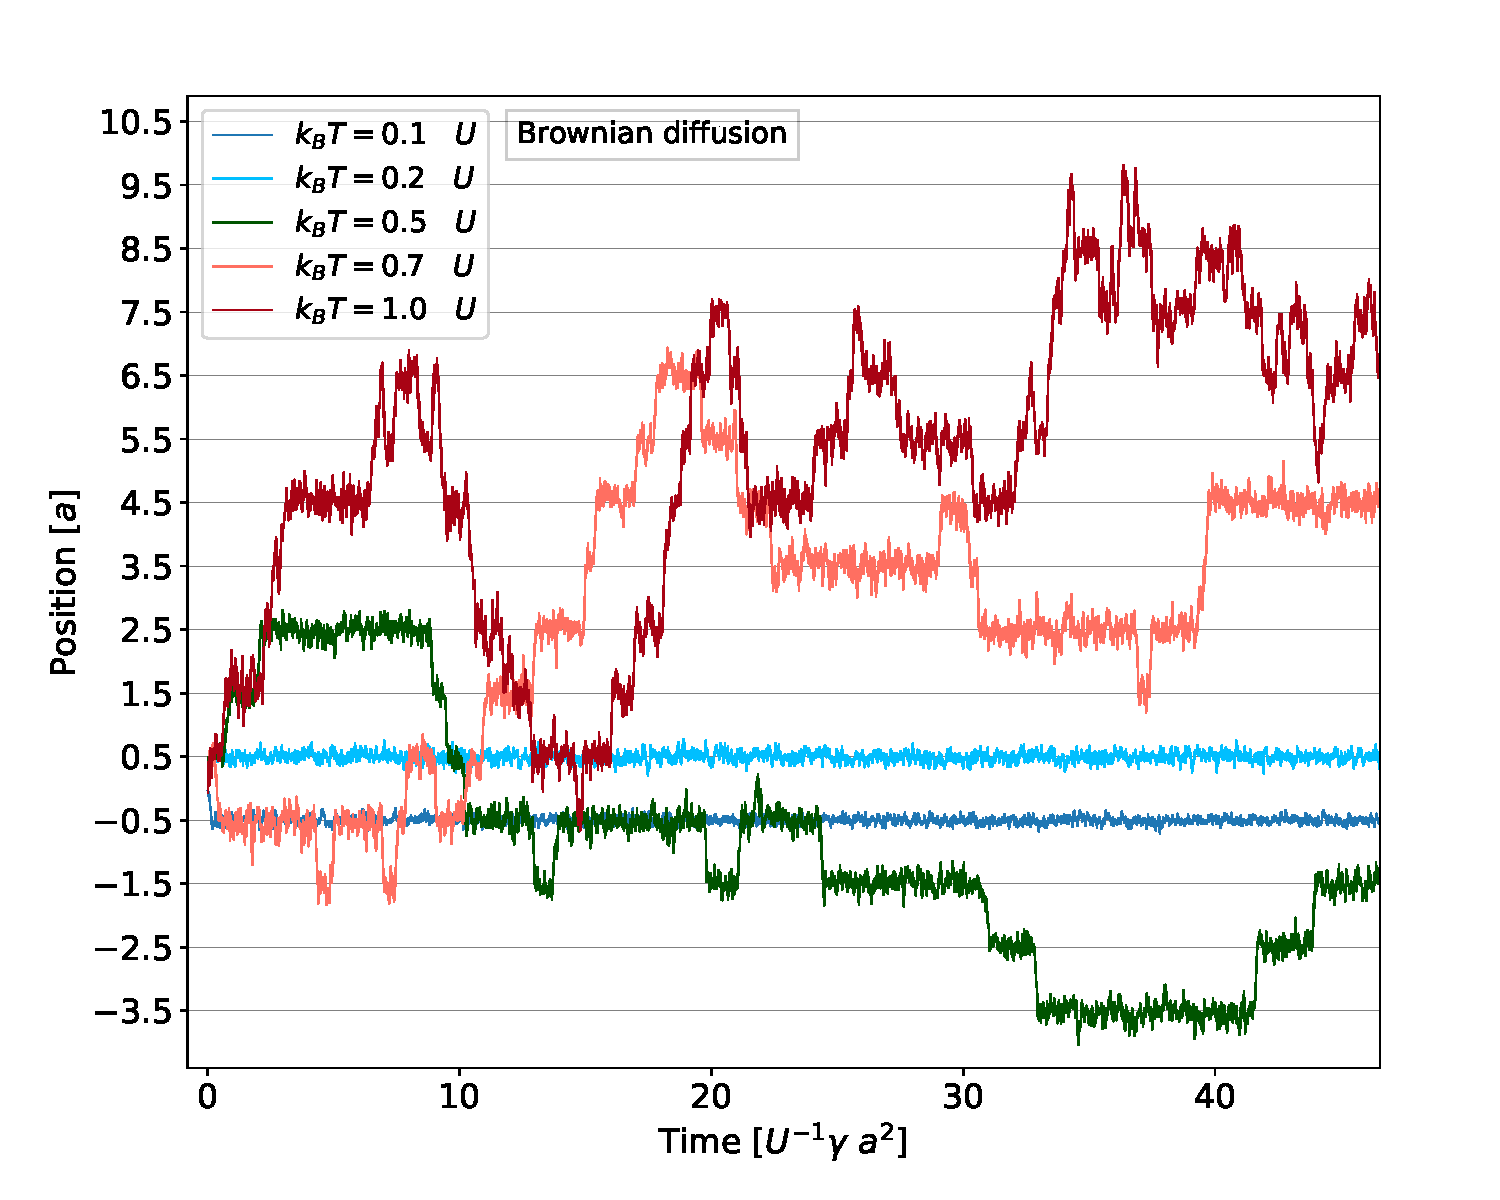
\includegraphics[width=0.9\textwidth]{scelta_temperatura.pdf}
\caption{Examples of solutions of the equation of motion \eqref{eq_def} started at $x(0)=0$, in no-driving conditions ($K=0\hspace{0.1cm}Ua^{-2}$) for a standard Brownian system ($k_b=0\hspace{0.1cm}Ua^{-2}$), at the few indicated values of temperature $T$ (standard thermal diffusion). The thin horizontal lines indicate the positions of the potential minima.}
\label{graph_Tchoice}
\end{figure}

Figure \ref{graph_Tchoice} reports the outcome of a few simulations of pure diffusion for a few different temperatures.
This figure illustrates how the particle moves under the competing effects of thermal fluctuations and of the sinusoidal corrugation potential.
\begin{itemize}[label={\scalebox{0.4}{$\blacksquare$}}]
    \item When $k_BT=0.1/0.2 \hspace{0.1cm}U$ the particle drops in one of the adjacent minima, then oscillates around the minimum position. Inter-minima thermally activated jumps are extremely rare.
    \item When $k_BT=0.5\hspace{0.1cm}U$ the random forces leave the particle at a minimum for the most of the simulation time, but are sufficiently strong to promote occasional jumps, and therefore a visible diffusive motion.
    \item When $k_BT=0.7 / 1\hspace{0.1cm}U$ minima and intermediate barriers are both significantly explored, the inter-minima jumps are so frequent that diffusive events dominate.
\end{itemize}
The time evolution for the non-Markovian model is qualitatively similar, but with less frequent inter-well jumps (see Fig.\;\ref{fig:T_kb15}).
\begin{figure}
    \centering
    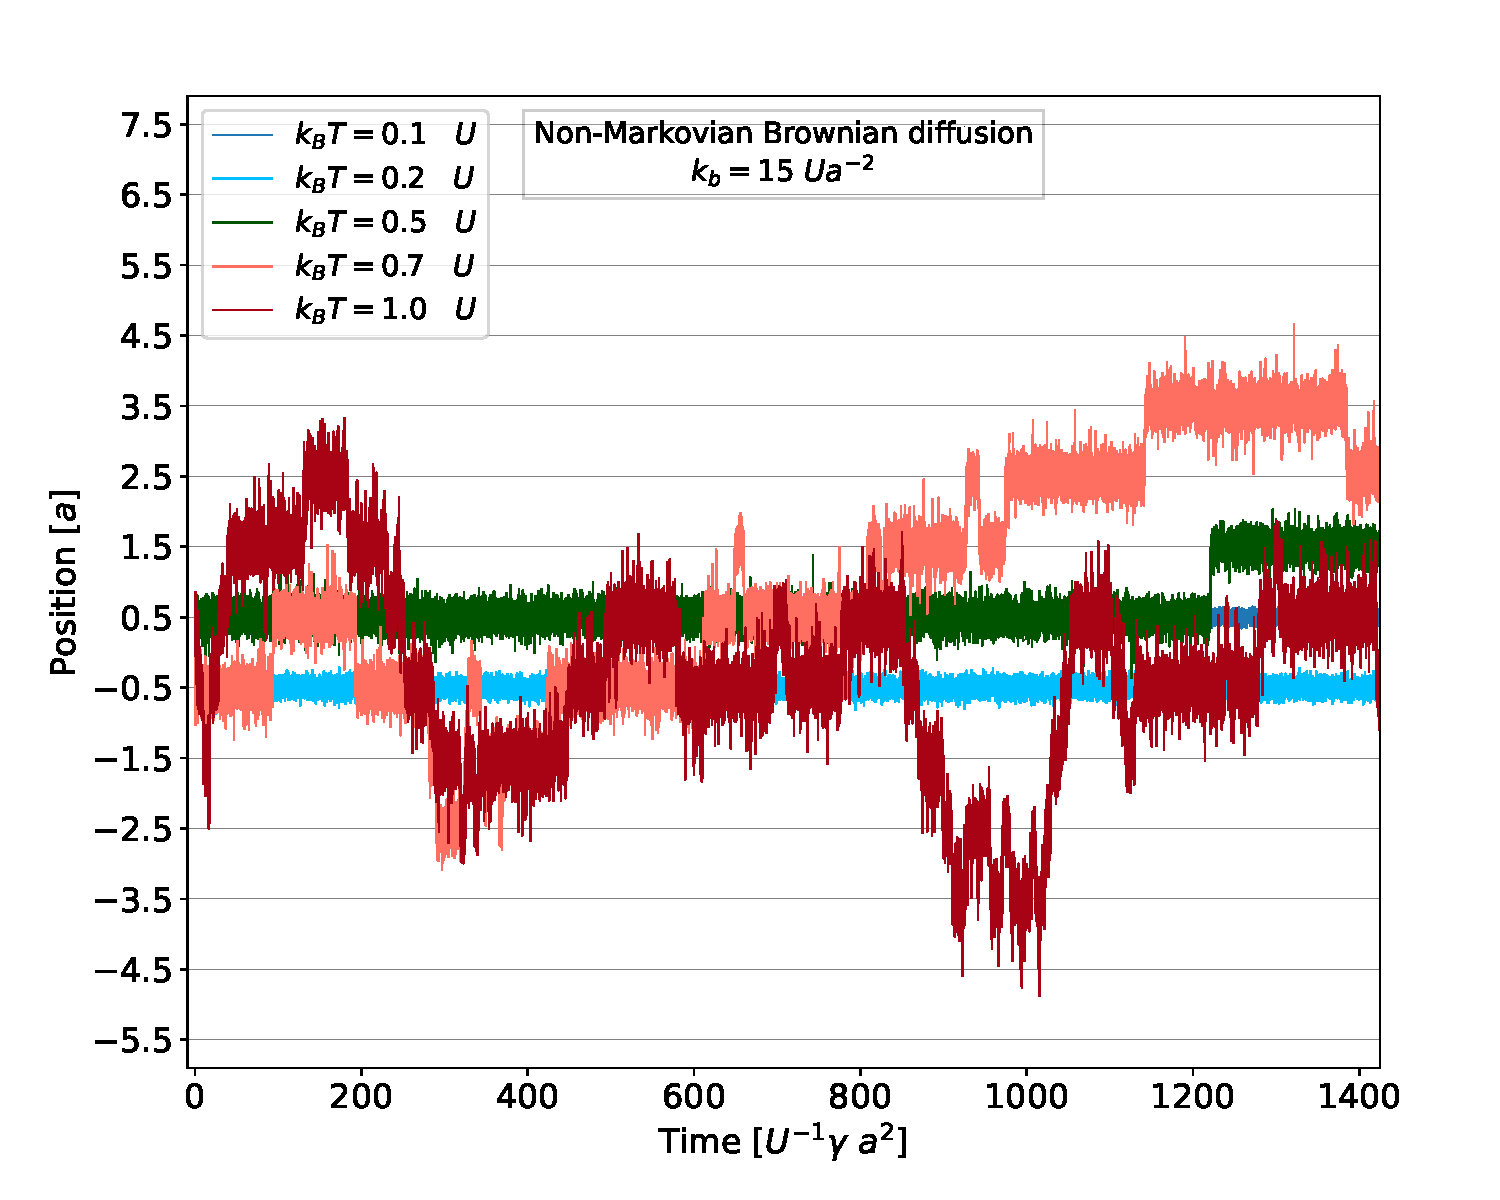
\includegraphics[width=0.9\textwidth]{scelta_temperatura_kb15.pdf}
    \caption{Same as Fig.\,\ref{graph_Tchoice}, but for a Brownian particle in a non-Markovian  environment with $k_b=15\; Ua^{-2}$}
    \label{fig:T_kb15}
\end{figure}
Since we are interested in studying the statistics of barrier jumps, we see that a suitable temperature is $k_BT = 0.5\hspace{0.1cm}U$, which is large enough that jumps occur at a fair rate, but not so large that the residence time at the potential wells becomes negligible.
\subsection{Damping coefficients and spring constants}
In this part, we refer to the experiments described in Ref.\cite{ginot2022} to tune the parameters used in our simulations. Specifically, Ref.\cite{ginot2022} employs damping coefficients $\gamma =\SI{0.186}{\micro\newton\second\meter^{-1}}$ and $\gamma_b = \SI{1.44}{\micro\newton\second\meter^{-1}}$. To adopt a similar ratio of viscous coefficients in our model, we consider  $\gamma_b = 7 \gamma$. With regard to the spring constant $k_b$, linking the true particle to the non-Markovian environment fake particle, to fix its value we identify the elastic energy accumulated in that spring when the true and fake particles sit at the bottom of adjacent wells. In the experiment of Ref.\cite{ginot2022}, a spring constant $k_b=\SI{0.4}{\micro\newton\meter^{-1}}$ is used. The distance between two minima is $2x_m =\SI{0.64}{\micro\meter}$ therefore the elastic energy is given by 
\begin{center}
    $U_{k_b} = \dfrac{1}{2}k_b (2 x_m)^2 \simeq 8.19 \cdot 10^{-20} \;\SI{}{J}$
\end{center}
The potential barrier in the model of Ref.\cite{ginot2022} 
\begin{center}
    $\Delta U = 2.1\hspace{0.1cm} k_BT \simeq 8.65 \cdot 10^{-21}\;\SI{}{\joule}$
\end{center}
because the experiments are conducted at $T=\SI{25}{\degreeCelsius}=\SI{298.15}{\kelvin}$. As a result 
\begin{center}
    $\dfrac{1}{2}\dfrac{k_b (2 x_m)^2}{\Delta U} \simeq 9.47$
\end{center}
To obtain a similar ratio in our model where the height of the potential barrier is twice of the natural units $\Delta U = U_0 = 2\hspace{0.05cm}U$. In our model, two consecutive minima are separated by a distance $a$; therefore, we can express the elastic energy as
\begin{center}
    $U_{k_b}  = \dfrac{1}{2}k_b a^2$
\end{center}
By comparing the quantities just described, we observe that the corresponding value of harmonic spring $k_b$ in our units would equal $37.9 \hspace{0.1cm} Ua^{-2}$, thus we explored comparable although slightly smaller values $k_b= 15 \hspace{0.1cm} Ua^{-2}$ and $k_b= 20 \hspace{0.1cm} Ua^{-2}$.

As for the elastic spring constant $K$, it describes how strongly the colloidal particle is coupled to the sliding stage. 
A very small value of $K$ implies that it may take several thousands of time units for the colloidal particle to start following the slider, thus a steady state may be hard to reach. On the other hand, with a large $K$ the particle would move close to the driving stage and thus may not exhibit significant effects of the interaction with the corrugation potential and the non-Markovian bath particle, as discussed for standard PT model in Section \ref{PTmodel}, and specifically around Eq.\eqref{eta}. As a fair compromise, for all driven simulations we adopt $K=0.001\hspace{0.1cm}Ua^{-2}$.
\subsection{Velocity}
The choice of the slider velocity $v$ range to investigate is based on the fact that it determines the particle's average waiting time $t_\text{w} = a/v$ in the potential minima. For the effects of the non-Markovian environment to be significant, we need $t_\text{w}$ to be comparable to or longer than the typical times between thermally-activated interwell jumps. As shown in Figure \ref{graph_Tchoice}, thermal jumps can occur every few times $t_0$ for $k_BT=0.5\hspace{0.1cm}U$. As a result, interesting physics is expected for 
\begin{center}
    $v \lesssim \dfrac{a}{10\hspace{0.1cm}t_0} = 0.1 \hspace{0.1cm} U a^{-1}\gamma^{-1}.$
\end{center}
On the other hand, a very low velocity would cause the slider to advance by only a few units of length $a$ even in very long simulations. For instance, at a velocity of $10^{-6}\; Ua^{-1}\gamma^{-1}$, the stage would move by one unit of length $a$ in a simulation with $t_\text{tot}=10^6\hspace{0.1cm}t_0$ that requires one billion time steps.
Extremely low velocities $v < 10^{-4} Ua^{-1}\gamma^{-1}$ although potentially useful to investigate the velocity-dependence of the friction force in the PT model and in its extension are too challenging for this preliminary study, and we will not attempt them.
\newpage
\chapter{Angular Observables and Correlations in Top-Pair Production}
We report our investigation of the dynamics of a colloidal particle in a Prandtl-Tomlinson setup, focusing on the effects of a non-Markovian environment. To make contact with Ref.\cite{ginot2022}, we begin our analysis by examining the dynamics of barrier crossing and the distributions of waiting times of the colloidal particle in a minimum. We conduct separate comparisons between pure, no driving, jump-diffusion with and without memory effects, as well as between the complete Prandtl-Tomlinson model and its non-Markovian extension. Finally, we compare the velocity-dependent behavior of the friction force between the standard PT model and its non-Markovian version.
\section{Effective potential}
In this section, we aim to begin understanding how a viscoelastic environment influences the motion of a colloidal particle threading a sinusoidal energy landscape. To achieve this, we first address the effective potential to which the particle is subjected in Brownian motion and its extension within a non-Markovian environment.

In these conditions, characterized by purely thermal effects, the probability distribution of the positions of a particle follows the Boltzmann equilibrium probability distribution.
\begin{equation}
    P(x) = \dfrac{1}{Z} e^{-\beta V_\text{eff}(x)}\, ,
\end{equation}
here $x$ denotes the position, $V_\text{eff}(x)$ the effective potential energy acting on the particle, $Z$ represents the partition function and $\beta =(k_B T)^{-1}$.
From this relation, we can express the effective potential as follows
\begin{equation}
    V_\text{eff}(x)=-k_BT \left(\log{Z} + \log{P(x)}\right)\, .
    \label{eq:potenz_efficace}
\end{equation}
Here the partition function $Z$ contributes just an irrelevant additive constant.
\begin{figure}
    \centering
    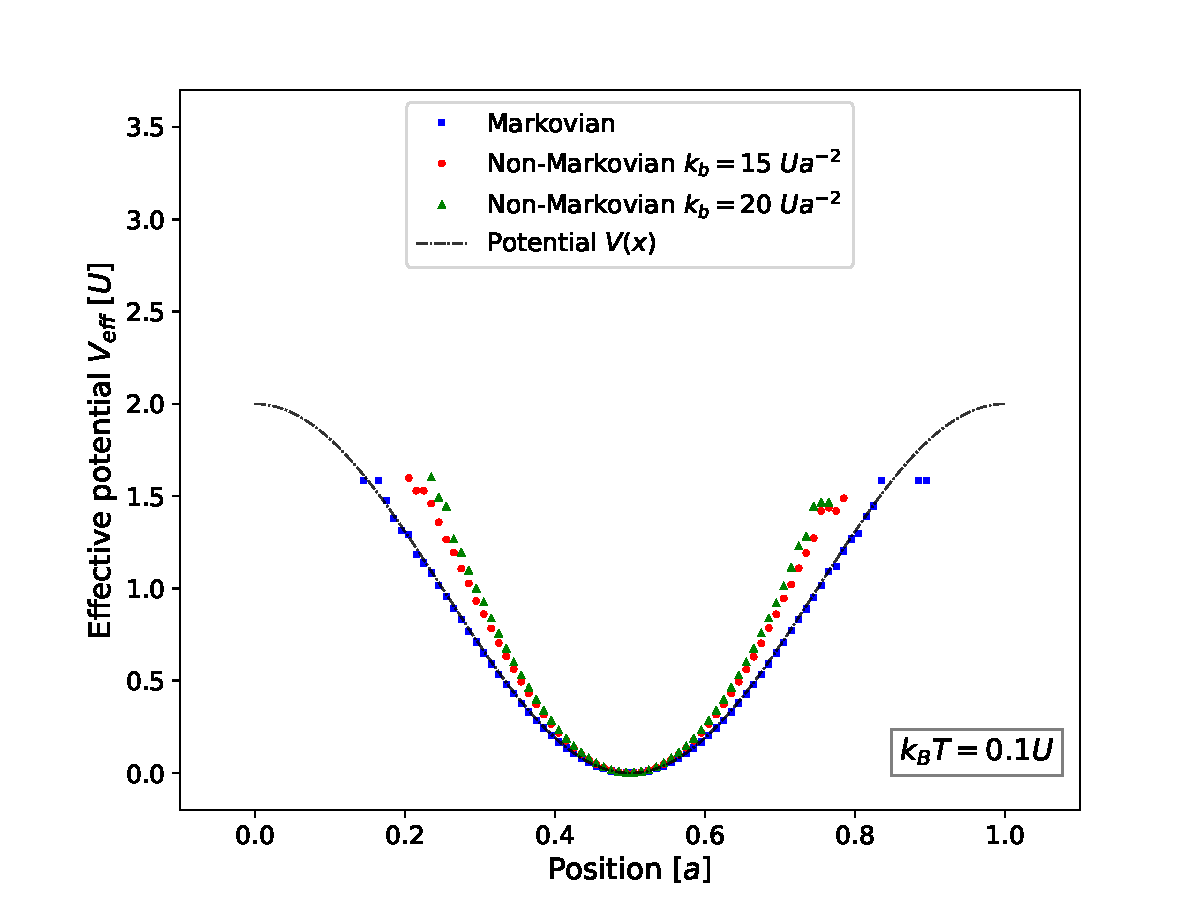
\includegraphics[width=\textwidth]{T01_U_eff.pdf}
    \caption{Comparison of the effective potential $V_\text{eff}(x)$ obtained through a histogram of the successive positions along a simulation at $k_BT=0.1\hspace{0.1cm}U$ through Eq.\eqref{eq:potenz_efficace}, for the standard Markovian environment ($k_b=0$) and two values of couplings $k_b$ to the memory bath. The actual potential, shifted so that its minimum coincides with the $k_b=0$ curve, is also shown as a dot-dashed line for comparison.}
    \label{fig:eff_pot_kbt01}
\end{figure}
To evaluate the probability distribution of the particle positions $P(x)$ we wrote a python script which maps the particle's position at successive simulation steps onto $0\leq x \leq 1\hspace{0.1cm}a$ of the corrugation potential and evaluate a 100-bins histogram of position occurences along the simulation. From the resulting normalized histogram, using relation \eqref{eq:potenz_efficace}, we reconstruct a map of the effective potential $V(x)$ experienced by the Brownian particle. Figure \ref{fig:eff_pot_kbt01} reports the resulting effective potential for the standard Markovian environment, and for 2 values of the coupling spring to the non-Markovian bath, evaluated for $k_BT=0.1\hspace{0.1cm}U$. At this low temperature, the Boltzmann factor at the maxima is $e^{-20} \simeq 2 \cdot 10^{-9}$ times smaller than at the minima, so even though the simulation cover $N=10^9$ steps, in practice the maxima are never explored, and this figure covers just the low-energy region near the minimum. Even with this drawback, it is apparent that in the presence of the non-Markovian thermostat, the effective potential experienced by the particle is steeper. We have also explored $k_BT=0.2\hspace{0.1cm}U$. At this higher temperature the regular Markovian bath has a relative Boltzmann probability of visiting the maximum that is $e^{-10} \simeq 4.5 \cdot 10^{-5}$ smaller than that of sitting at a minimum. In this condition, indeed, the Brownian particle is able to explore all the points of the potential, occasionally reaching the maxima in simulations of $10^9$ steps. However, this practically never occurs in the presence of a non-Markovian environment. For this reason, we raise the temperature to $k_BT=0.5\hspace{0.1cm}U$, allowing the model to explore the maxima of the potential a sufficient number of times for accumulating a significant statistics. 
\begin{figure}[ht!]
    \centering
    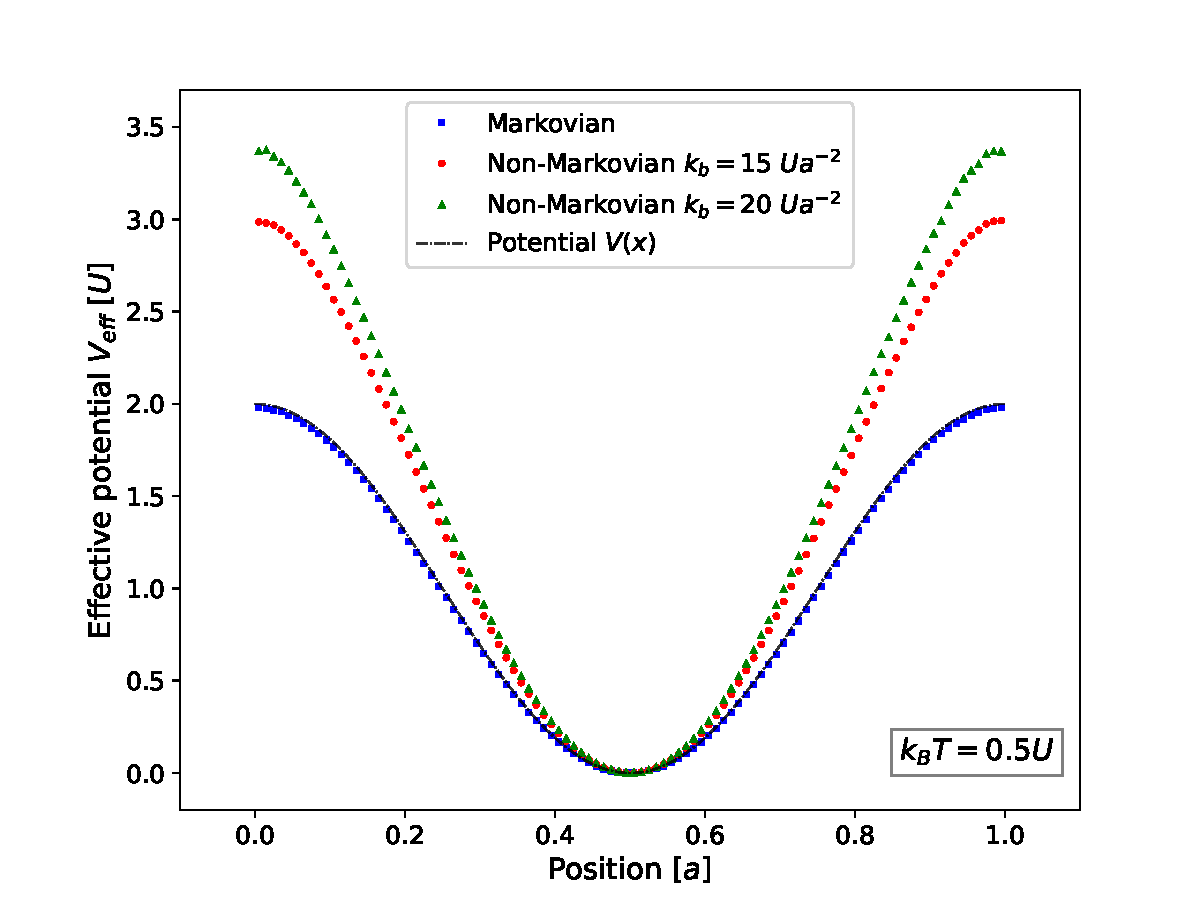
\includegraphics[width=\textwidth]{T05_U_eff.pdf}
    \caption{Same as Fig. \ref{fig:eff_pot_kbt01}, but for a substantially higher $k_BT=0.5\hspace{0.1cm}U$}
    \label{fig:effpotenz}
\end{figure}
\\
Figure \ref{fig:effpotenz} perfectly illustrates that for a simple Brownian particle, the effective potential $V_\text{eff}(x)$ coincides exactly with the corrugated potential on which it moves. Furthermore, it is observed that the effect of the viscoelastic non-Markovian environment is to raise the potential barrier while leaving the position of the minimum unchanged at $x=0.5\hspace{0.1cm}a$, thus making it much steeper. These simulations are carried out for $10^9$ time steps to ensure a sufficient number of counts in each bin, thus correctly sampling the effective potentials $V_\text{eff}(x)$.
\section{Waiting-time distribution}
To gain deeper insights into the motion of a colloidal particle across a viscoelastic bath in this section we investigate the barrier-crossing dynamics of a particle under various conditions. Initially we are going to study the dynamics of barrier crossing under pure Brownian non-driven conditions, followed by a study of this statistics for the full Prandt-Tomlinson model. 
\begin{figure}[ht!]
    \centering
    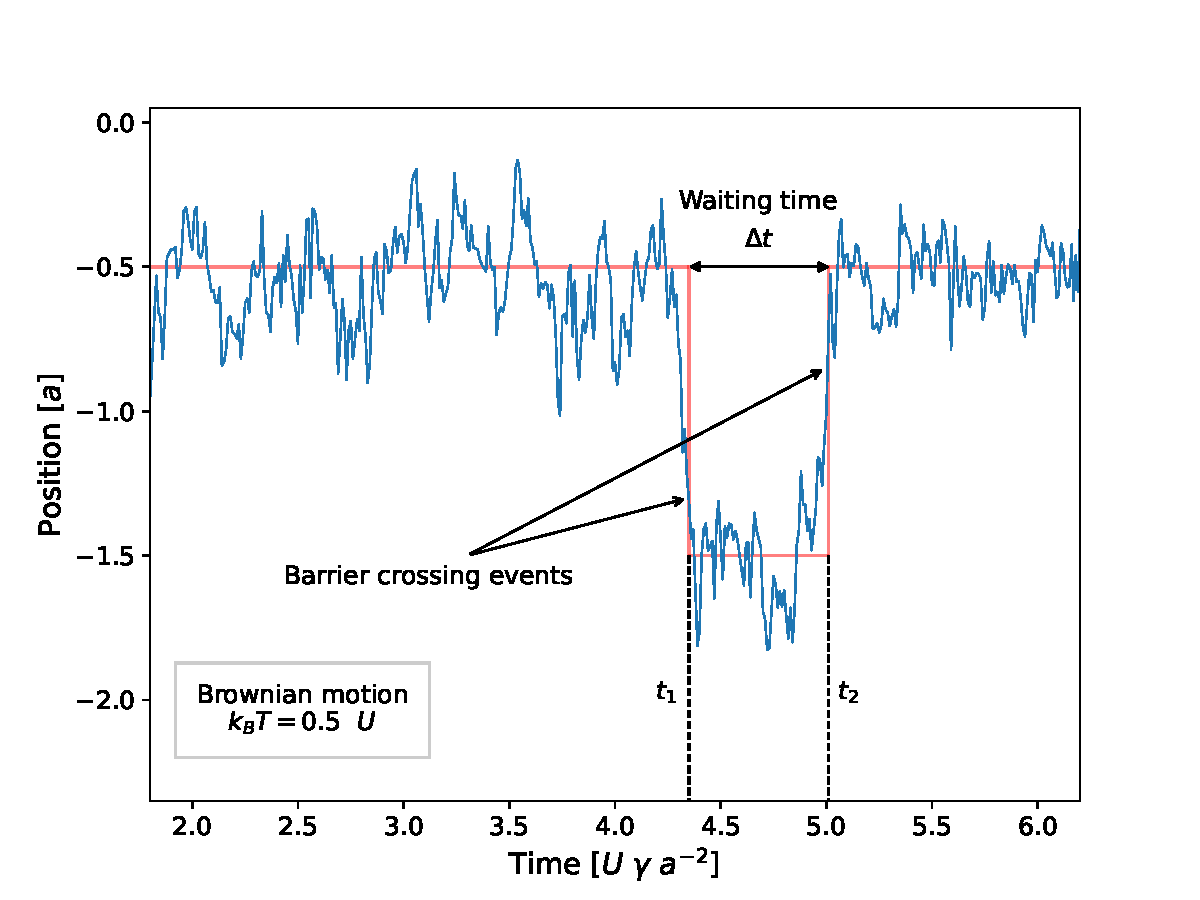
\includegraphics[width=\textwidth]{definition_barrcross2.pdf}
    \caption{Visual definition of barrier crossing event and waiting time}
    \label{fig:definition_barrcross}
\end{figure}
\\
Firstly, let us define a barrier-crossing event as the instant when the particle's displacement reaches at least $x = 0.7 \hspace{0.1cm}a$ from the current minimum.
This condition assures us that the colloidal particle definitely left the minimum and has transitioned into one of the adjacent minima. Moreover we define the waiting time as the duration between two consecutive crossing events, see Fig.~\ref{fig:definition_barrcross}.
To analyze barrier-crossing events and waiting times we have developed a python code to calculate the probability distribution $P(t_\text{w})$ of waiting times $t_\text{w}$ in the minima. This probability distribution $P(t_\text{w})$ is developed through a histogram characterized by a variable bin width allowing us to capture a fair detail of the short timescale and to ensure an adequate number of points to produce a fair statistics of long waiting times. The histogram is adequately normalized to $1$ to allow a fair comparison of different trends, in a correctly-normalized probability density.
\subsection{Brownian motion and non-Markovianity}\label{sec_markov_vs_non}
In this part we compare simple Brownian diffusion with diffusion in a viscoelastic bath. As previously explained, Brownian diffusion characterises the stochastic movement of a particle suspended in a fluid due only to time-independent memory-free effects and collisions with surrounding particles of the fluid. When the surrounding medium is a viscoelastic fluid, the environment generates memory effects keeping track of previous particle positions.

Figure \ref{P_kb15} shows a comparison between the probability distributions of waiting times $P(t_\text{w})$ of simple Brownian diffusion ($k_b=0$, triangles) and $P(t_\text{w})$ in the non-Markovian environment simulated with $k_b=15\hspace{0.1cm}Ua^{-2}$ (squares). For these simulations we consider $k_BT=0.5 \hspace{0.1cm}U$.
\begin{figure}[h!]
    \centering
    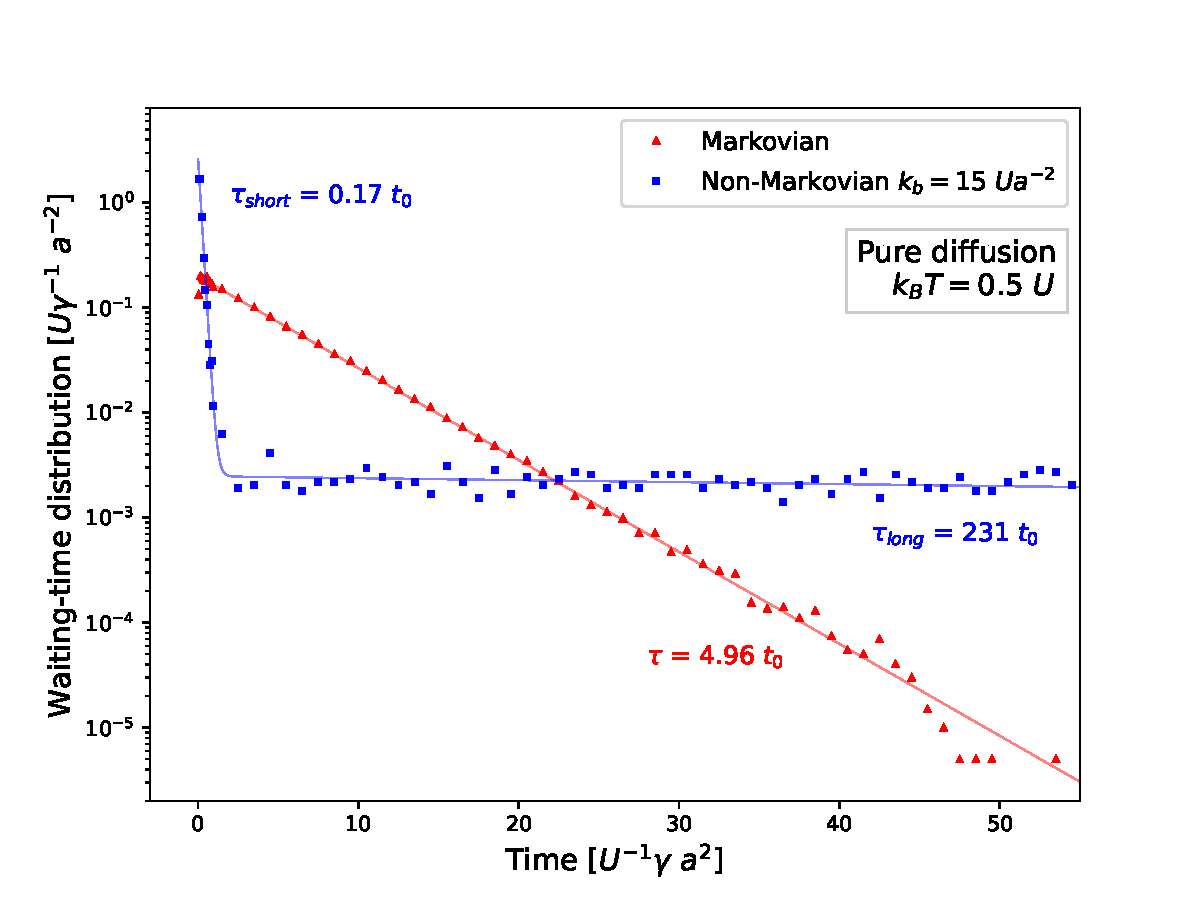
\includegraphics[width=\textwidth]{kb15_T05.pdf}
    \caption{Comparison of the waiting-time distributions of a simple Brownian particle and the same particle in a non-Markovian environment ($k_b=15\hspace{0.1cm}Ua^{-2}$), both simulated at $k_BT = 0.5\hspace{0.1cm}U$}
    \label{P_kb15}
\end{figure}
\\
In Figure \ref{P_kb15} the histograms are characterized by a variable bin width: $0.1\hspace{0.1cm}t_0$ from $0$ to $1$ and $1\hspace{0.1cm}t_0$ from $1$ to $100$.
\\
As suggested by the lin-log scale, the probability distribution of waiting times in the ordinary Markovian environment $P_{k_b=0}(t_\text{w})$ follows an exponential decay in the form 
\begin{equation}
    P_{k_b=0}(t_\text{w})= A \exp{\left(- \dfrac{t_\text{w}}{\tau}\right)}\,.
    \label{eq:P_kb0}
\end{equation}
The solid line in Fig. \ref{P_kb15} is a fit of the histogram points, obtained using an appropriate NumPy function. Table \ref{tab:fit_brownian_diffusion} presents the best fit parameters $A$ and $\tau$.
\begin{table}[ht]
\centering 
\begin{tabular}{cc}
    \toprule
    Parameter & Value  \\
    \midrule 
    $\tau \hspace{0.1cm} [t_0]$ & $4.96\pm 0.05$ \\[0.5ex]
    $A \hspace{0.1cm} [t_0^{-1}]$ & $0.20\pm 0.01$ \\
    \bottomrule
\end{tabular}
\caption{Best fit parameters of the waiting-time distribution $P(t_\text{w})$, Eq.\eqref{eq:P_kb0}, for the standard, Markovian thermostat inducing Brownian diffusion.}
\label{tab:fit_brownian_diffusion}
\end{table}
\\
\noindent The waiting-time statistics for the Brownian particle with memory is remarkably different: Figure \ref{P_kb15} shows that the probability distribution exhibits a double exponential decay with two different time scales: a short timescale associated to back-and-forth events with the particle being recalled into the originating minimum shortly after the jump due to viscoelastic effects, and a long timescale corresponding to regular diffusive processes. To evaluate the relative time scales, we decide to lead us to fit the delay times with the sum of two exponential decays in the following form:
\begin{equation}
    P(t_\text{w}) = A_\text{short} \exp{\left(- \dfrac{t_\text{w}}{\tau_\text{short}}\right)} + A_\text{long} \exp{\left(- \dfrac{t_\text{w}}{\tau_\text{long}}\right)}\,.
\end{equation}
Table \ref{tab:fit_brownian_withmemory} reports the coefficients obtained and the associated errors.
\begin{table}
\centering 
\begin{tabular}{ccc}
    \toprule
    Fit parameter & $k_b=15\hspace{0.1cm}[Ua^{-2}]$& $k_b=20\hspace{0.1cm}[Ua^{-2}]$\\
    \midrule 
    $\tau_\text{short} \hspace{0.1cm} [t_0]$ & $0.17\pm 0.01$ & $0.13 \pm 0.01$\\[0.5ex]
    $A_\text{short} \hspace{0.1cm} [t_0^{-1}]$ & $2.6 \pm 0.4$ & $0.0012 \pm 0.0001$\\[0.5ex]
    $\tau_\text{long} \hspace{0.25cm} [t_0]$ & $231 \pm 12$ & $460 \pm 93$\\[0.5ex]
    $A_\text{long} \hspace{0.2cm} [t_0^{-1}]$ & $ 0.0025 \pm 0.0001$ & $5 \pm 2$\\
    \bottomrule
\end{tabular}
\caption{Parameters of waiting-time distributions $P(t_\text{w})$ for Brownian diffusion with memory effects of Figs. \ref{P_kb15} 
 ($k_b=15\hspace{0.1cm}Ua^{-2}$) and \ref{P_kb20} 
 ($k_b=20\hspace{0.1cm}Ua^{-2}$), both simulated at $k_BT=0.5\hspace{0.1cm}U$ }
\label{tab:fit_brownian_withmemory}
\end{table}
\\
Figure \ref{P_kb20} reports similar results for a stiffer viscoelastic thermostat ($k_b=20\hspace{0.1cm}Ua^{-2}$). Comparing Figs. \ref{P_kb15} and \ref{P_kb20}, we can observe how the viscoelastic bath, and thus the memory of the environment, influences the distribution of waiting times in the potential minima. In particular, we observe that the Brownian motion with memory supports even very long waiting times of hundreds of time units, as opposed to the regular Markovian thermostat, for which long waiting times in excess of a few tens of time units are radically suppressed at the explored temperature. In the short-times region, the viscoelastic rapid-recall mechanism has the distribution of non-Markovian waiting times exceed that of the regular Markovian bath. In contrast, in the $0.3\hspace{0.1cm}t_0 \lesssim t_\text{w} \lesssim t_0$ range, the regular Markovian dynamics leads to more likely delay times.
\begin{figure}
    \centering
    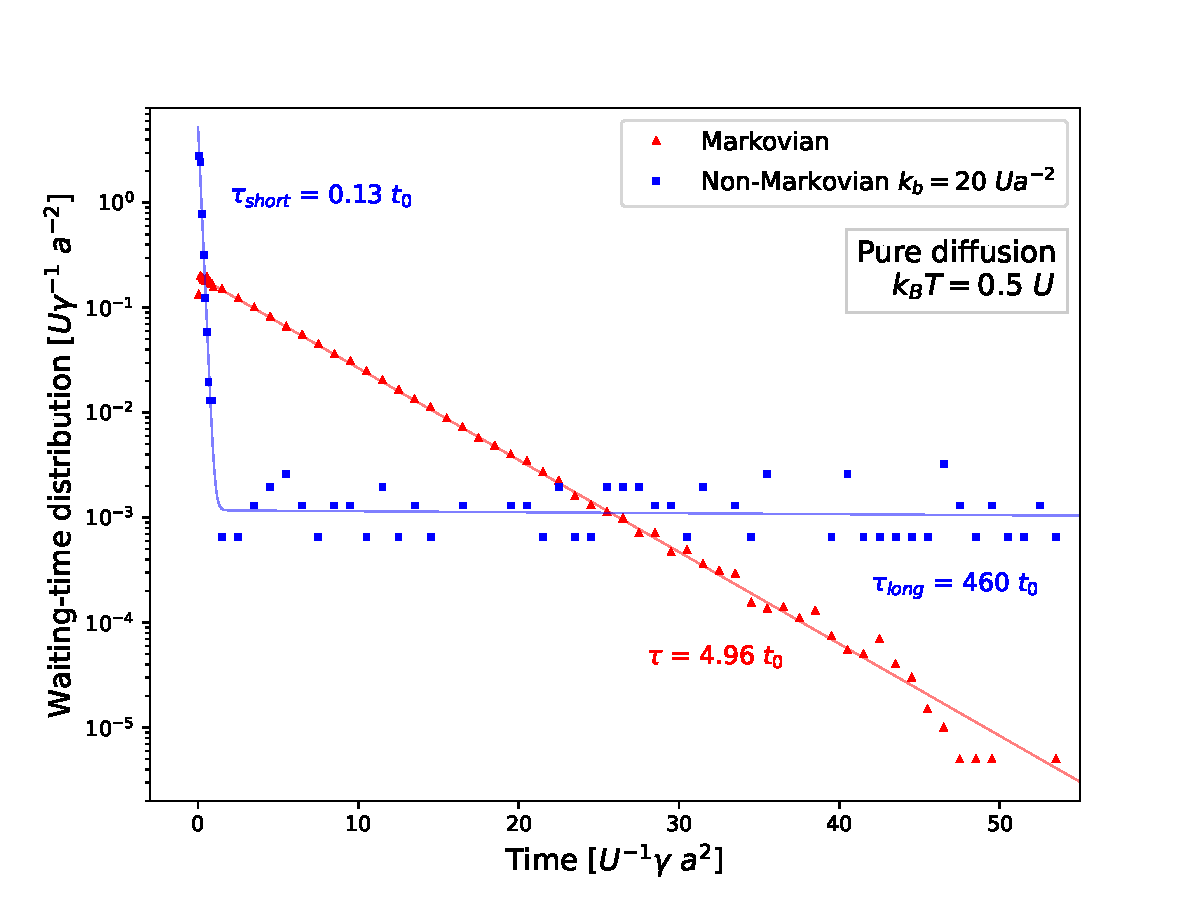
\includegraphics[width=\textwidth]{kb20_T05.pdf}
    \caption{Same as Figure \ref{P_kb15}, but for a viscoelastic spring $k_b=20\hspace{0.1cm}Ua^{-2}$}
    \label{P_kb20}
\end{figure}
Note that in Figure \ref{P_kb20} the histograms have a different bin width compared to those in Figure \ref{P_kb15}, more precisely, a bin width of $2\hspace{0.1cm}t_0$ is set from $1\hspace{0.1cm}t_0$ onwards. This is because, with a higher coupling constant $k_b$, the number of barrier crossing events is lower, requiring the merging of more times to obtain useful statistics.
\clearpage
\subsection{Temperature effect on Brownian motion}
Here we investigate how temperature influences the waiting-time distributions $P(t_\text{w})$. In particular, to study this effect, we compare the waiting-time distributions of a simple Brownian particle and a Brownian particle with memory when $k_BT=0.7\; U$.
\begin{figure}[ht!]
    \centering
    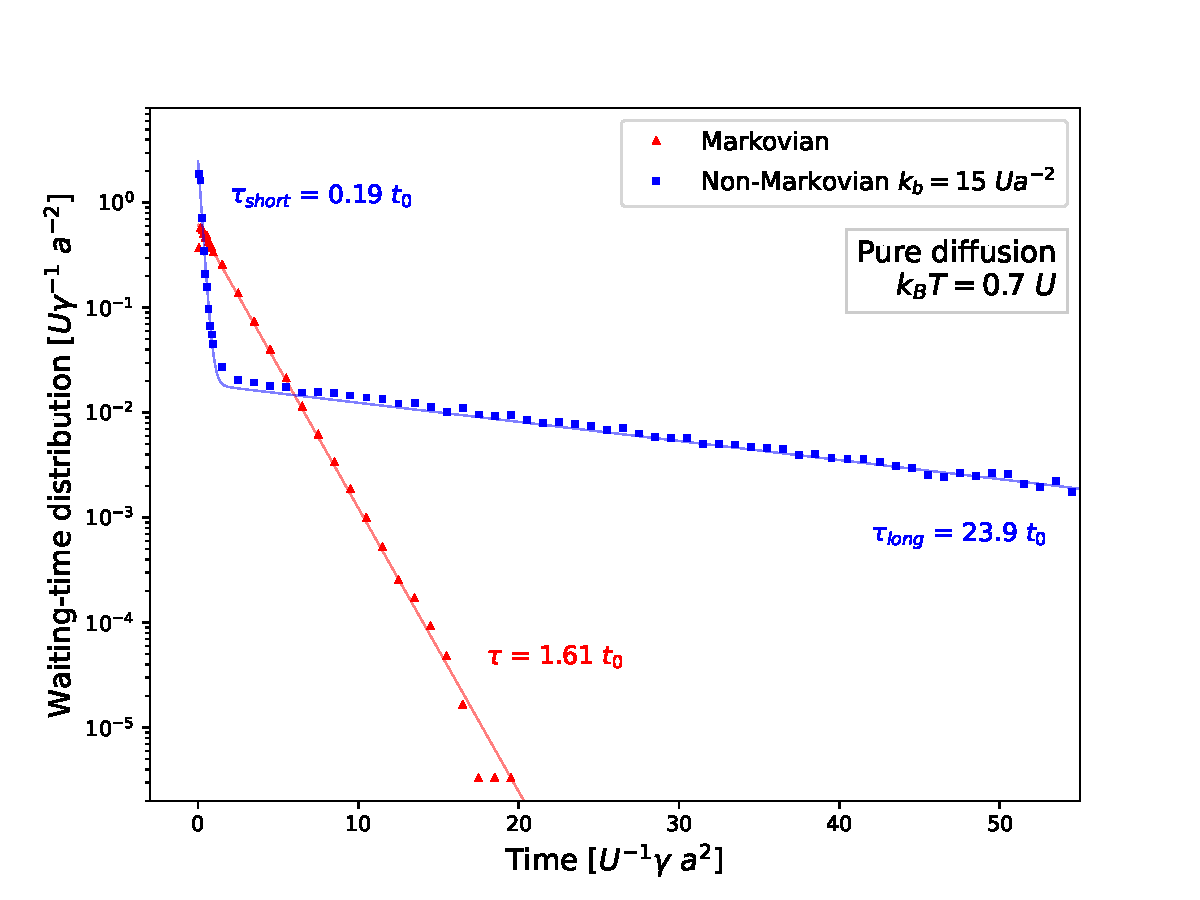
\includegraphics[width=0.9\textwidth]{kb15_T07.pdf}
    \caption{Same as Fig.~\ref{P_kb15}, but for $k_BT = 0.7\hspace{0.1cm}U$}
    \label{fig:kb15_temp_high}
\end{figure}
In both scenarios the decays exhibit shorter characteristic times $\tau$ compared to lower temperature $k_BT=0.5\; U$. $\tau_\text{long}$ is significantly affected, while $\tau_\text{short}$ remains nearly the same, as it is mainly affected by the viscoelastic spirng $k_b$. This effect is due to the presence of larger stochastic forces, causing the particle to exit the potential minima more rapidly.
\begin{table}
\centering 
\begin{tabular}{ccc}
    \toprule
    Fit parameter & $k_BT = 0.5\hspace{0.1cm}U$ & $k_BT = 0.7\hspace{0.1cm}U$ \\
    \midrule
    $\tau_\text{short} \hspace{0.1cm} [t_0]$ & $0.171\pm 0.009$ & $0.19 \pm 0.01$\\[0.5ex]
    $\tau_\text{long} \hspace{0.25cm} [t_0]$ & $221 \pm 12$ & $23.9 \pm 0.3$\\[0.5ex]
    
    
    \bottomrule
\end{tabular}
\caption{Comparison of characteristic times of Brownian diffusion with memory $k_b=15\hspace{0.1cm}Ua^{-2}$ of two different temperatures}
\label{tab:variando_kbt}
\end{table}
\clearpage
\subsection{Standard Prandtl-Tomlinson model}
\label{sec:spiegobinning}
We come now to investigate the distribution of waiting times $P(t_\text{w})$ for the standard Prandtl-Tomlinson model, i.e. without considering a viscoelastic environment($k_b=0$), but including driving through a spring with $K=10^{-3}\hspace{0.1cm}Ua^{-2}$. In these simulations $k_BT$ is set to $0.5\hspace{0.1cm}U$.
\begin{figure}
    \centering
    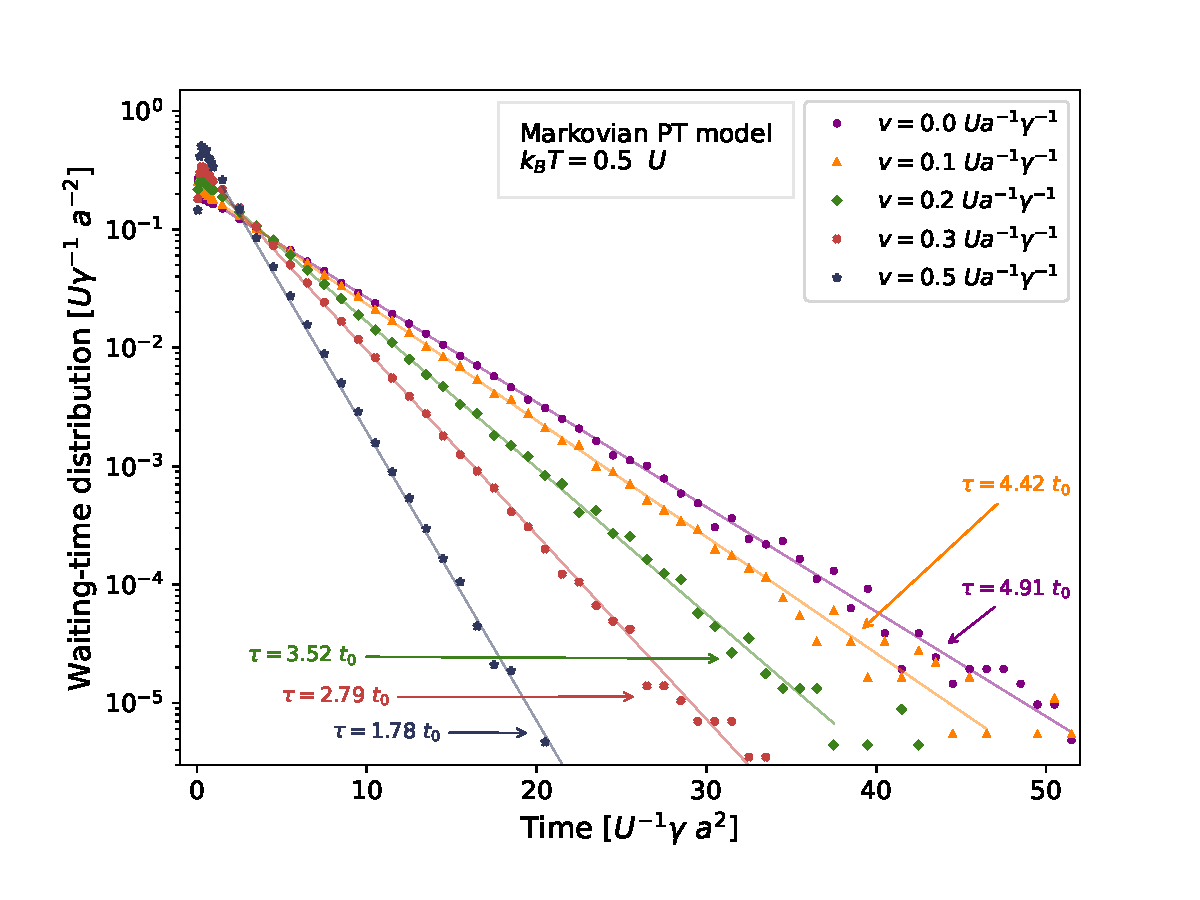
\includegraphics[width=\textwidth]{standard_PT_definitivo.pdf}
    \caption{Waiting times distribution $P(t_\text{w})$ of a standard PT model ($k_b=0$) for a few values of the the sliding velocity $v$ and fixed parameters $K=0.001\, Ua^{-2}$ and $k_BT=0.5\hspace{0.1cm}U$.}
    \label{fig:simplePT}
\end{figure}
\\
Figure \ref{fig:simplePT} reports a few histograms of the standard PT model driven at few different velocities. The $v=0$ simulation yields the distribution of waiting times of a simple Brownian particle constrained with a spring of elastic constant $K$ to a fixed point: this is similar to the free model, and we take it as the reference to compare the $v>0$ simulations. The waiting-time distributions exhibit long timescale exponential decays with decreasing characteristic time values $\tau$ as a function of $v$. This is expected since a larger slider velocity reduces the probability of longer waiting times favoring shorter stays in the potential minima.
\begin{table}
\centering 
\begin{tabular}{cc}
    \toprule
    Velocity $v$ [$U \gamma ^{-1} a^{-1}$] & Fit parameter $\tau$ [$t_0$]  \\
    \midrule 
    $0.0$ & $4.91\pm 0.04$\\
    $0.1$ & $4.42 \pm 0.04$ \\
    $0.2$ & $3.52\pm 0.02$\\
    $0.3$ & $2.79\pm 0.02$ \\
    $0.5$ & $1.78 \pm 0.03$ \\
    \bottomrule
\end{tabular}
\caption{Parameters of waiting times distribution $P(t_\text{w})$ for standard Prandtl-Tomlinson model}
\label{tab:simplePT}
\end{table}
Table \ref{tab:simplePT} reports the characteristic times $\tau$ obtained through a linear fit over the natural logarithms of bin heights, performed using the appropriate NumPy function. The fitting is performed from the first bin after the peak in the distribution to the one before the first empty bin, beyond which data become unreliable. This protocol of bin range for fitting single exponential decays is also applied to all subsequent fits.

\subsection{Non-Markovian Prandtl-Tomlinson model}
In this section we aim to understand how the distributions of waiting times in potential minima change when considering our non-Markovian Prandtl-Tomlinson model compared to the regular PT model under analogous driving conditions.
\begin{figure}
    \centering
    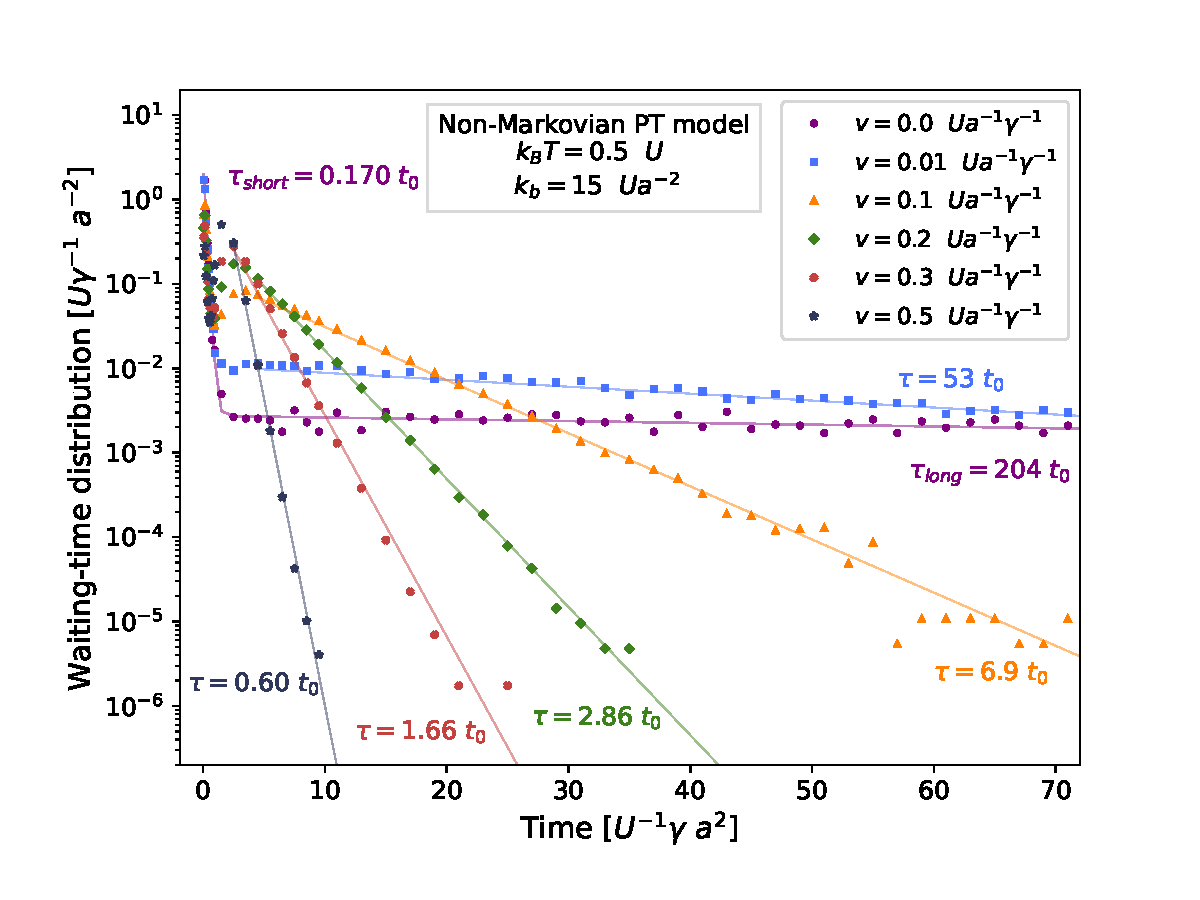
\includegraphics[width=0.9\textwidth]{istogramma_confronto_kb15_def.pdf}
    \caption{Same as Fig.~\ref{fig:simplePT} but for the non-Markovian thermostat, characterized by $k_b=15\hspace{0.1cm}Ua^{-2}$}
    \label{fig:confronto_velocità_kb15}
\end{figure}
Figure \ref{fig:confronto_velocità_kb15} reports six distributions of waiting times as a function of the slider velocity, from $0$ to $0.5 \hspace{0.1cm} U a^{-1} \gamma^{-1}$, while fixing the coupling parameters $k_b=15\hspace{0.1cm}Ua^{-2}$. The figure also reports the values of large-$t_\text{w}$ decay times $\tau$ for each distribution. These values are obtained following the same protocol described in Subsection \ref{sec:spiegobinning}. Like for the Markovian model, increasing the slider velocity results in fewer occurrences of longer waiting times. It may also be observed that, as $v$ increases, the waiting time distributions, after a rapid exponential decay at short timescales, related to the viscoelastic rapid back-and-forth events, exhibit an non monotonic trend characterised by a peak followed by the typical exponential decay at longer timescales. This peak becomes more pronounced and shifts to lower $t_\text{w}$ as the dragging velocity increases, as can be seen in the detail of the waiting-time distributions reported in Figure \ref{fig:zoom_kb15}.
\begin{figure}
    \centering
    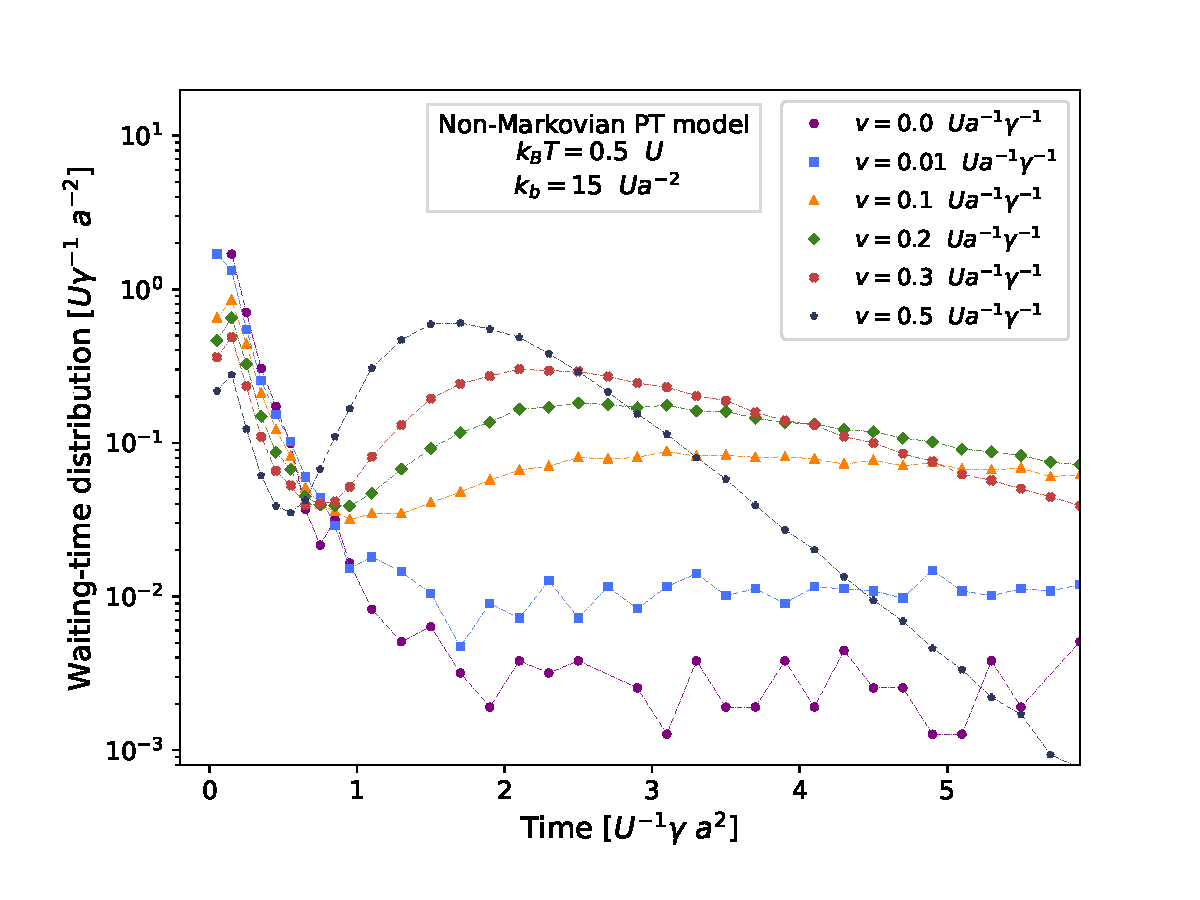
\includegraphics[width=0.9\textwidth]{zoom_kb15.pdf}
    \caption{Detail of Fig. \ref{fig:confronto_velocità_kb15} using a bin width of $0.1\hspace{0.1cm}t_0$, from $0$ to $t_0$, and $0.2\hspace{0.1cm}t_0$ onward}
    \label{fig:zoom_kb15}
\end{figure}
\newpage
In particular, the formation of this peak is due to the presence of a characteristic waiting time $t_\text{ave}$ in a minimum, namely the average time between two consecutive minima at the dragging velocity $v$
\begin{equation}
    t_\text{ave} = \dfrac{a}{v}\, ,
\end{equation}
namely the inverse of the washboard frequency of the PT model.

Figure \ref{fig:confronto_velocità_kb20} shows the same comparison as Figure \ref{fig:confronto_velocità_kb15} using a different value of the viscoelastic coupling spring $k_b=20\hspace{0.1cm}Ua^{-2}$.
\begin{figure}
    \centering
    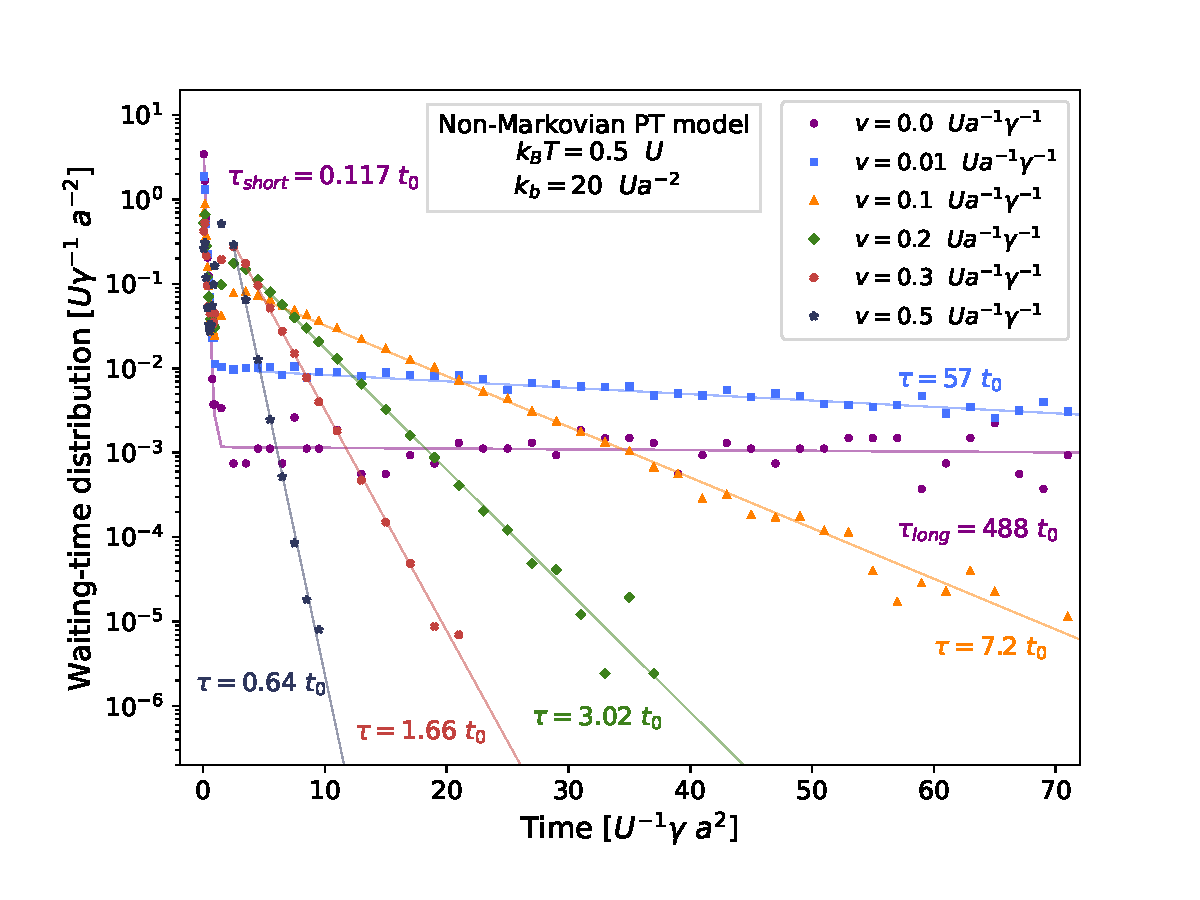
\includegraphics[width=\textwidth]{istogramma_confronto_kb20_def.pdf}
    \caption{Same as Fig.~\ref{fig:confronto_velocità_kb15}, but for $k_b=20\hspace{0.1cm}Ua^{-2}$.}
    \label{fig:confronto_velocità_kb20}
\end{figure}
The effect of a stronger coupling with the viscoelastic bath is to keep the particle for longer times in the potential minima, consistent with higher effective barriers see Fig.~\ref{fig:effpotenz}. Comparing $k_b=15\hspace{0.1cm}Ua^{-2}$ and $k_b=20\hspace{0.1cm}Ua^{-2}$, the characteristic times $\tau$ undergo minor changes, see also Table \ref{tab:tau}.
\begin{table}
\centering 
\begin{tabular}{ccc}
    \toprule
    Velocity [$U \gamma ^{-1} a^{-1}$] & \multicolumn{2}{c}{Fit parameter $\tau$  [$t_0$]} \\
    \cmidrule(lr){2-3}
    & $k_b = 15$  [$Ua^{-2}$]& $k_b = 20$  [$Ua^{-2}$] \\
    \midrule 
    $0.01$ & $52.8\pm 0.9$ & $57 \pm 1$\\
    $0.1$ & $6.9 \pm 0.2$ & $7.2 \pm 0.1$\\
    $0.2$ & $2.86\pm 0.04$ &$3.02 \pm 0.09$\\
    $0.3$ & $1.66\pm 0.06$  &$1.66 \pm 0.02$\\
    $0.5$ & $0.60 \pm 0.02$  &$0.64 \pm 0.02$\\
    \bottomrule
\end{tabular}
\caption{Large-$t_\text{w}$ decay time of the distribution $P(t_\text{w})$ for the non-Markovian Prandtl-Tomlinson model and two different viscoelastic couplings $k_b$.}
\label{tab:tau}
\end{table}
\begin{figure}
    \centering
    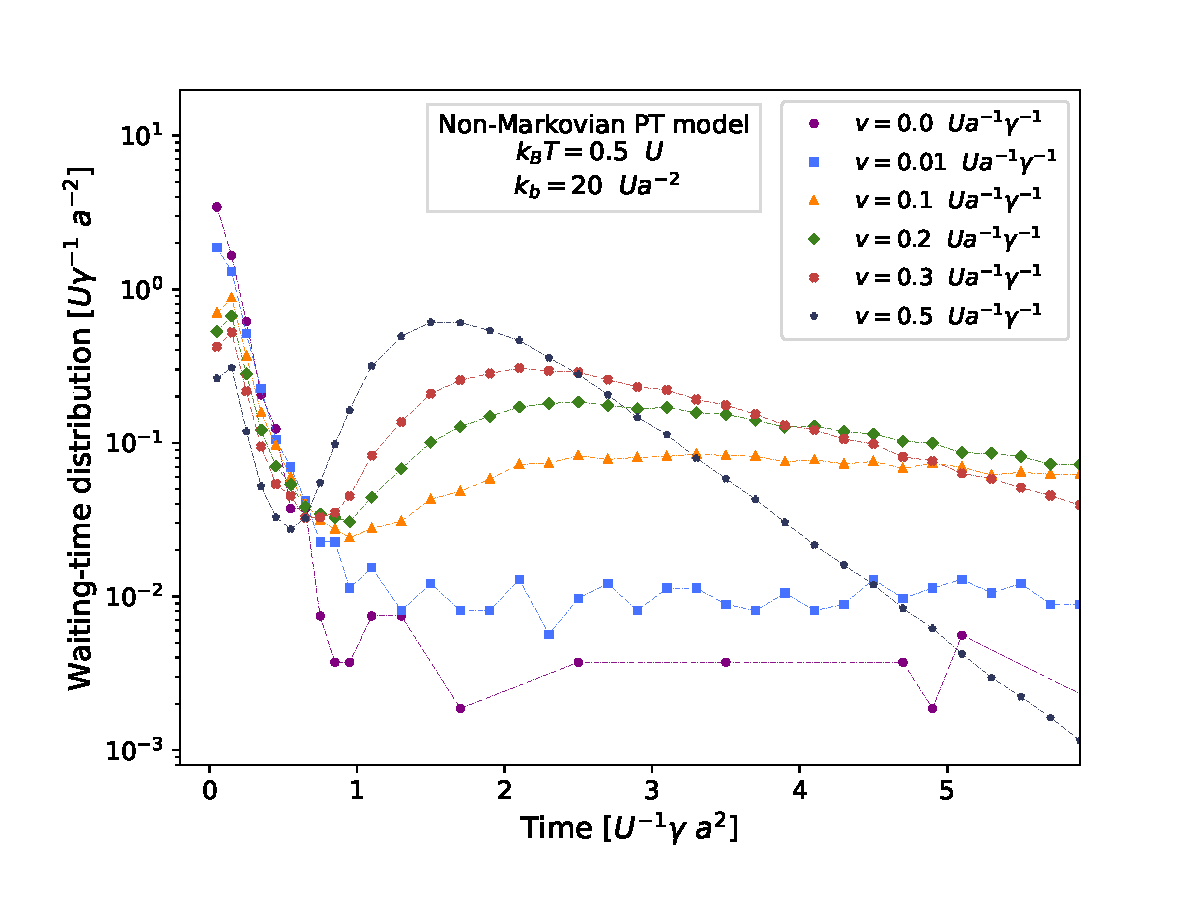
\includegraphics[width=\textwidth]{zoom_kb20.pdf}
    \caption{Same as Fig.~\ref{fig:zoom_kb15}, but for $k_b=20\, Ua^{-2}$.}
    \label{fig:zoom_kb20}
\end{figure}
\clearpage
\subsection{Left and right barrier crossings}
It is instructive to separately examine the distributions of crossings made to the left (backward) and to the right (forward). We define the right crossing waiting time as the waiting time in a minimum before a forward crossing occurs, namely a displacement of at least $0.7\hspace{0.1cm}a$ forward. The left crossing waiting time is defined similarly.

In particular, it is interesting to analyze left and right crossings waiting times by varying the velocity from $0$ to $0.5 \hspace{0.1cm} U a^{-1} \gamma^{-1}$. As expected, for zero velocity the distributions are practically identical, which is consistent with the fact that, under 'no-sliding' conditions, there is no preferred direction for barrier crossings, and they are evenly distributed in both directions due to thermal fluctuations.
\begin{figure}[ht!]
    \centering
    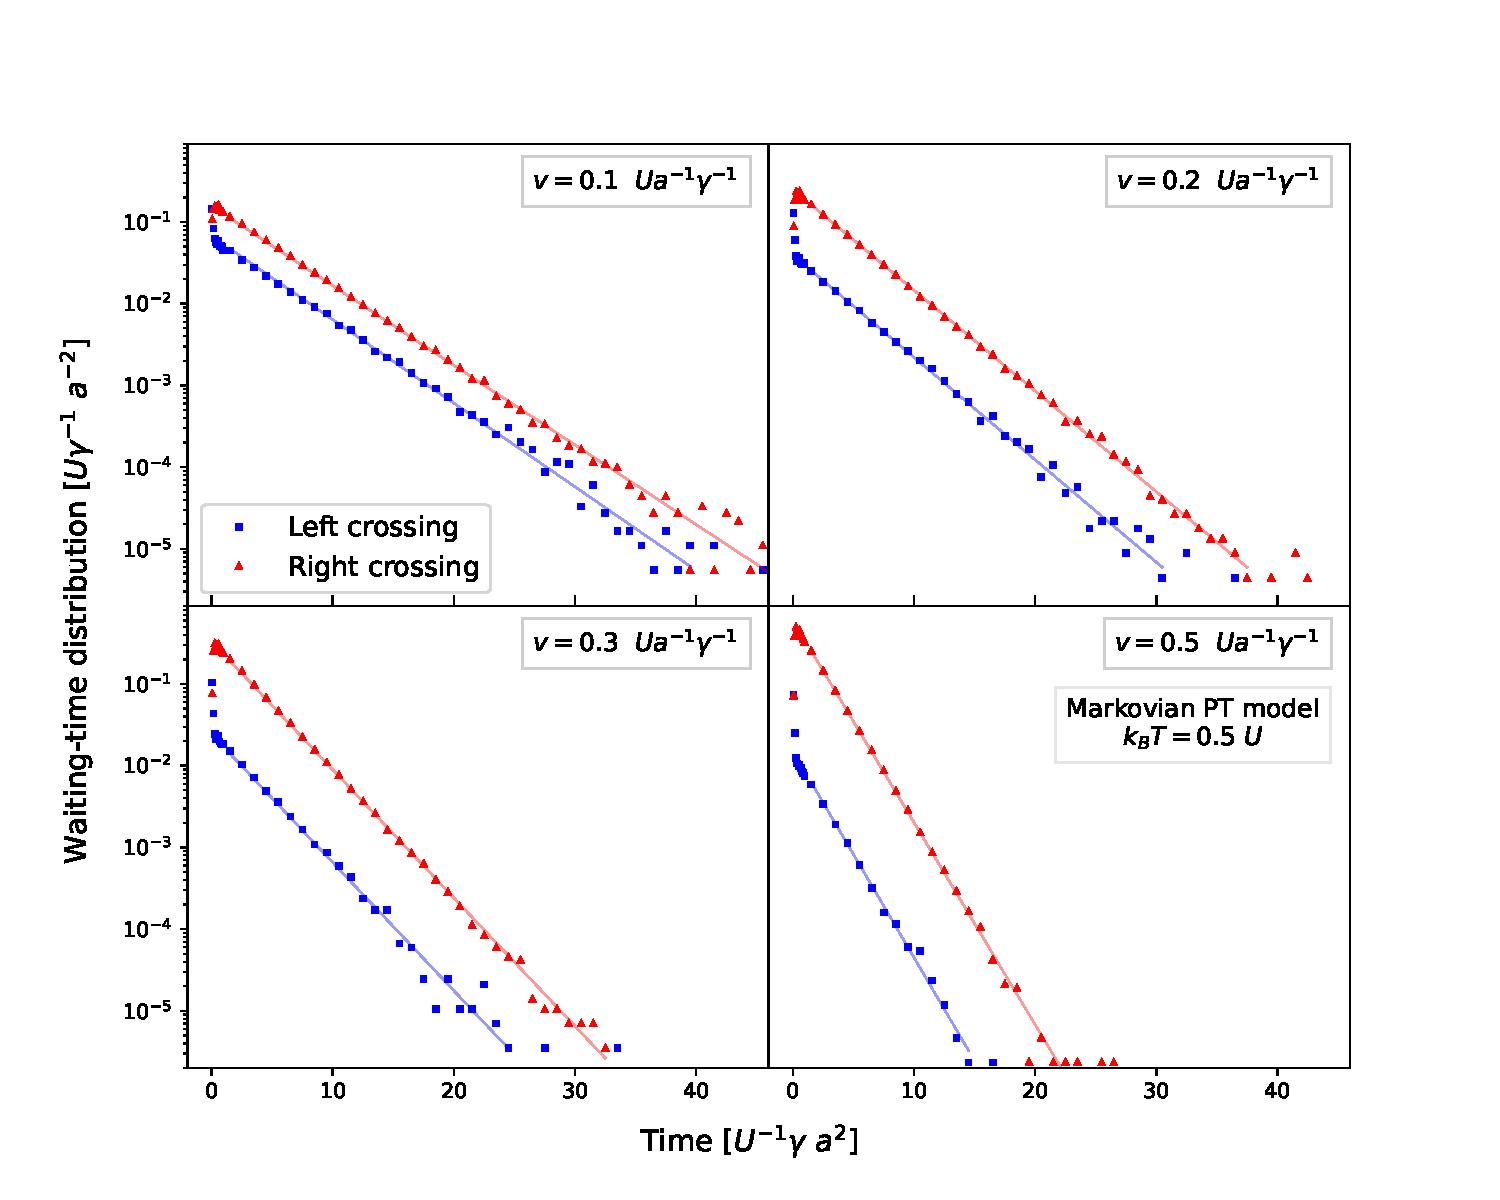
\includegraphics[width=\textwidth]{sxdx_simplePT_DEFINITIVO.pdf}
    \caption{Leftward (squares) and rightward (triangles) barrier crossings waiting-time distributions $P(t_\text{w})$ for the standard Markovian Prandtl-Tomlinson model for a few values of driving velocity $v$}
    \label{fig:simplePT_sxdx}
\end{figure}

The standard Prandtl-Tomlinson model exhibits decreasing similar characteristics times, but different ratios of barrier-crossing events as $v$ is increased, thus a different value of the prefactor. In both distributions the longer waiting times are suppressed as $v$ is increased, see Table \ref{tab:sxdx_simplePT}.
\begin{table}
\centering 
\begin{tabular}{ccc}
    \toprule
    Velocity [$U \gamma ^{-1} a^{-1}$] & Leftward $\tau_\text{left} $[$t_0$] & Rightward $\tau_\text{right} $[$t_0$]\\
    \midrule 
    $0.1$ & $4.24 \pm 0.07$ & $4.46 \pm 0.08$\\
    $0.2$ & $3.47 \pm 0.06$ & $3.52 \pm 0.02$ \\
    $0.3$ & $2.77 \pm 0.09$ & $2.77 \pm 0.03$\\
    $0.5$ & $1.71\pm 0.04$ & $1.77 \pm 0.04$\\
    \bottomrule
\end{tabular}
\caption{Characteristic times for the leftward and rightward-jumps waiting-time distribution $P(t_\text{w})$ for the Markovian Prandtl-Tomlinson model.}
\label{tab:sxdx_simplePT}
\end{table}

\begin{figure}
\centering
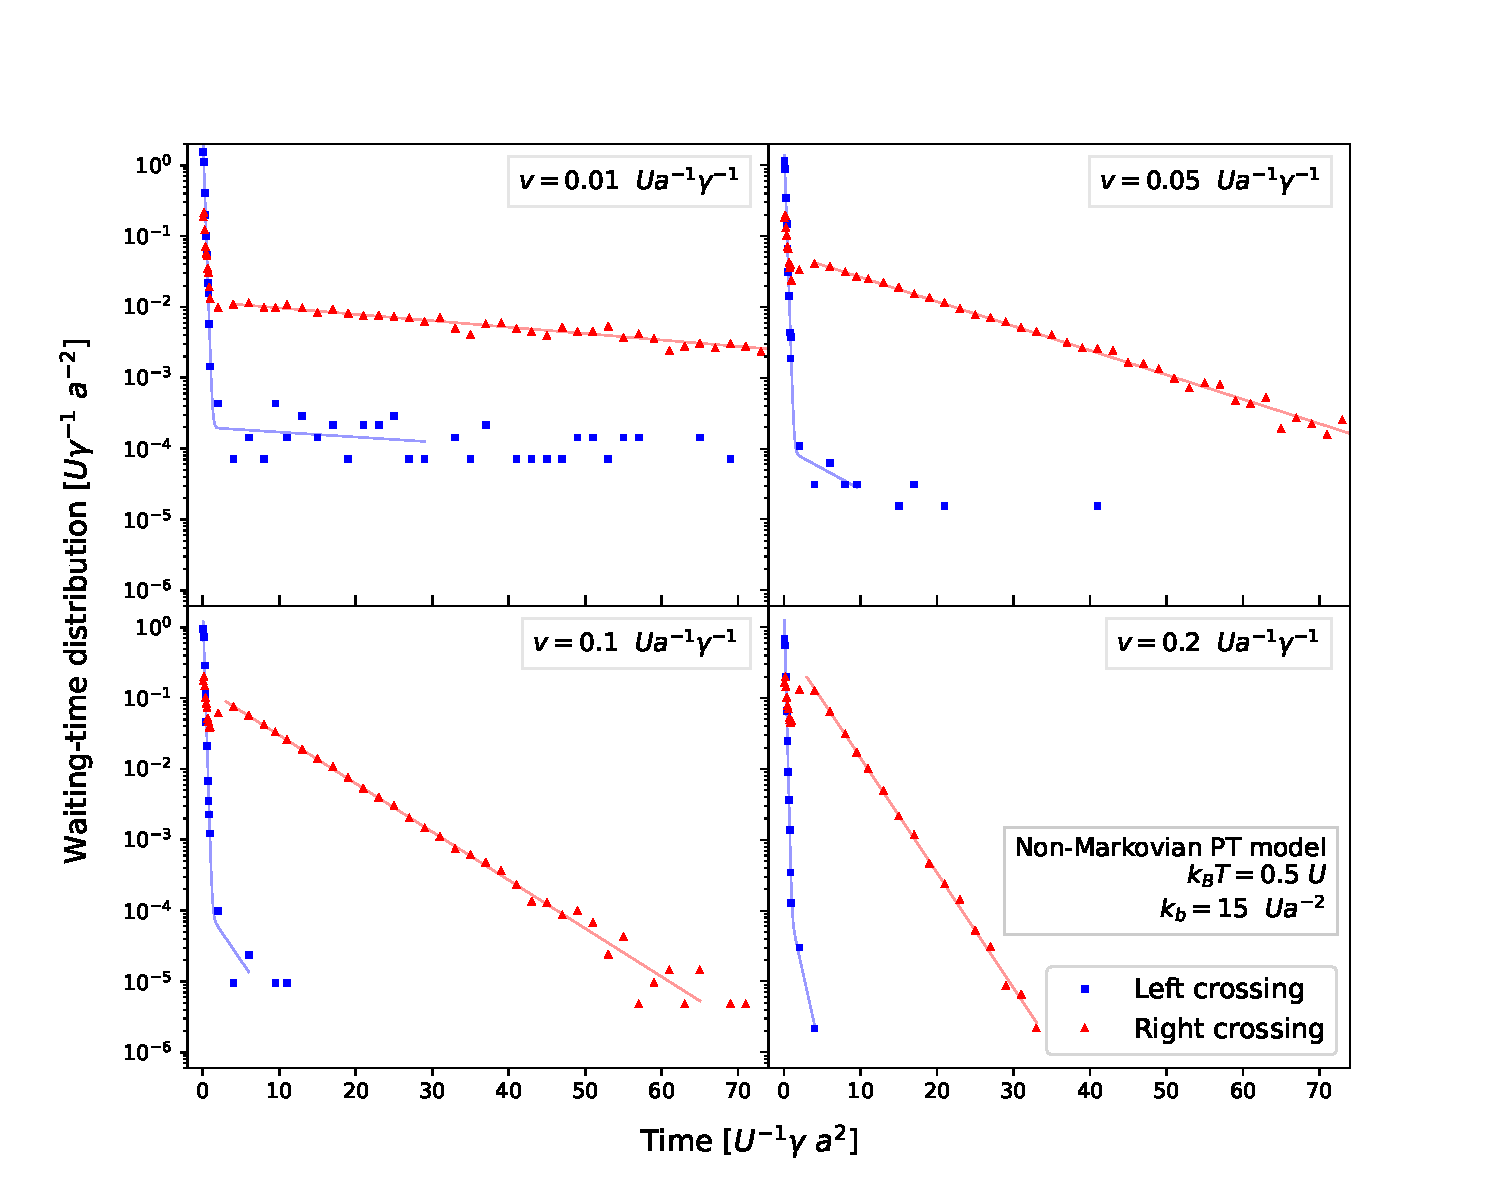
\includegraphics[width=\textwidth]{isto_sxdx_kb15_basseV.pdf}
\caption{Same as Fig. \ref{fig:simplePT_sxdx} but for the non-Markovian Prandtl-Tomlinson model with $k_b=15\; Ua^{-2}$.}
\label{fig:sxdx_kb15_basseV}
\end{figure}
The non-Markovian PT model instead develops a radical asymmetry in the left versus right distributions, even at moderate speed. Specifically, we notice two very different behaviors when considering the waiting time preceding a right barrier crossing compared to that of a left crossing. When the crossing is performed to the right, the characteristic time decreases as the velocity of the slider increases. However, for the left crossing, the characteristic time remains relatively similar and much shorter than that of the rightward jumps. For the rightward distributions we execute a linear fit over the logarithm of the right-crossing waiting-time distribution, which shows a single exponential decay on the long timescale. In contrast we fit the left crossing waiting-time distribution with a short timescale a sum of two exponentials. To evaluate whether the left crossing waiting times distribution exhibits a double exponential decay,
we computed the waiting-time distribution from $v=0.01\; Ua^{-1}\gamma^{-1}$ to $v=0.5\; Ua^{-1}\gamma^{-1}$.

Note that the histograms in Figure \ref{fig:simplePT_sxdx} have a bin width of $0.1 t_0$ from $0$ to $ t_0$, and then $t_0$ onwards. Instead, the histograms in Figures \ref{fig:sxdx_kb15_alteV} and \ref{fig:sxdx_kb15_basseV} have the same bin width, as Figure \ref{fig:simplePT_sxdx}, in the initial region, but in the $t_\text{w}>t_0$ region, they have different widths. For the histograms of waiting times before a rightward crossing, the bin width is set to $1 t_0$, while for the leftward waiting times, we adopt a bin width of $2 t_0$ to collect more of these rarer events, resulting in a sufficient number of data points for a fair statistics.
\begin{figure}
    \centering
    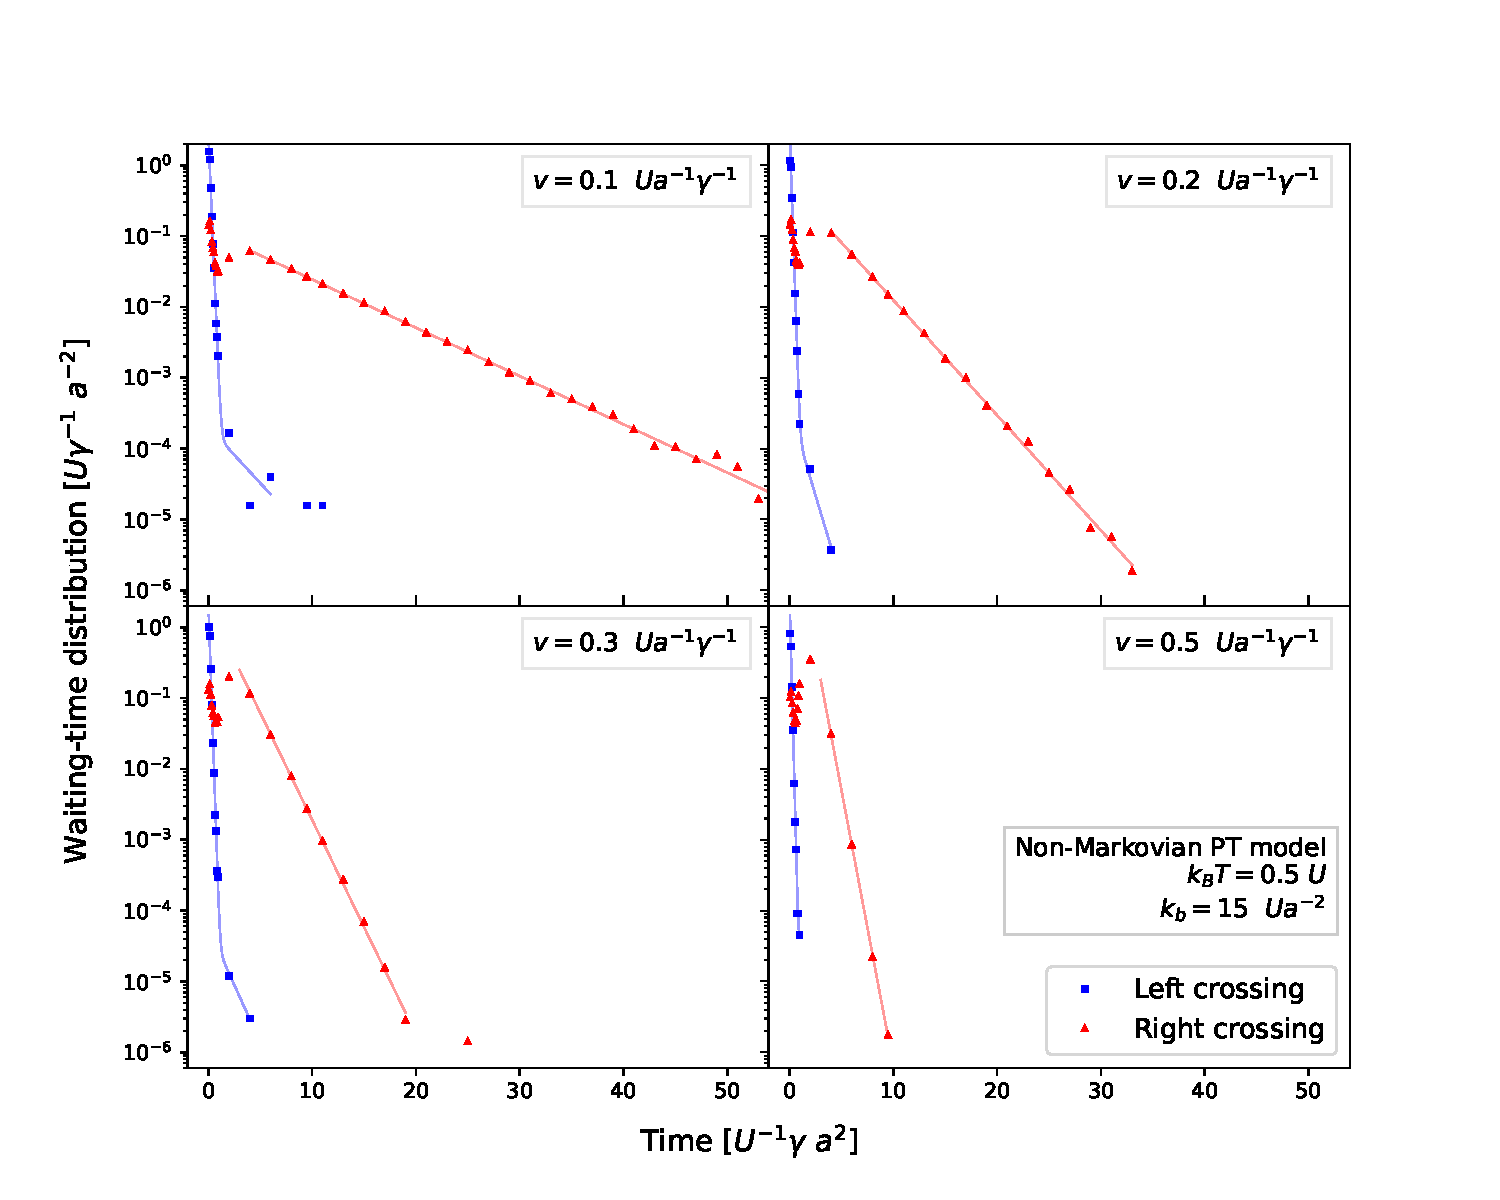
\includegraphics[width=\textwidth]{isto_sxdx_kb15_alteV.pdf}
    \caption{Same as Fig. \ref{fig:sxdx_kb15_basseV} but for higher velocities.}
    \label{fig:sxdx_kb15_alteV}
\end{figure}
\newpage
\noindent In Figure \ref{fig:sxdx_kb15_basseV}, we observe the double exponential decay of the waiting times distribution more clearly at lower speeds. Additionally, at slow driving the particle can remain for tens of time units before performing a leftward barrier crossing. Table \ref{tab:sxdx_right} reports the obtained characteristic times for the exponential decays of the rightward crossing waiting-time distribution
\begin{table}
\centering 
\begin{tabular}{ccc}
    \toprule
    Velocity [$U \gamma ^{-1} a^{-1}$] & Fit parameter $\tau $[$t_0$] \\
    \midrule 
    $0.01$ & $47.9 \pm 0.9$\\
    $0.05$ & $12.6 \pm 0.3$\\
    $0.1$ & $6.4 \pm 0.1$ \\
    $0.2$ & $2.67 \pm 0.03$ \\
    $0.3$ & $1.44 \pm 0.02$ \\
    $0.5$ & $0.560 \pm 0.006$ \\
    \bottomrule
\end{tabular}
\caption{Characteristic times for the rightward-jumps waiting-time distribution $P(t_w)$ for non-Markovian Prandtl-Tomlinson model with $k_b=15\; Ua^{-2}$}
\label{tab:sxdx_right}
\end{table}
\\Table \ref{tab:sxdx_left} reports the characteristic times for the two-exponential decays of the leftward crossing waiting times distribution
\begin{table}
\centering 
\begin{tabular}{ccc}
    \toprule
    Velocity [$U \gamma ^{-1} a^{-1}$] & Fit parameter $\tau_{short} [t_0]$ & Fit parameter $\tau_{long} [t_0]$ \\
    \midrule 
    $0.01$ & $0.13 \pm 0.01$ & $63 \pm 17$\\
    $0.05$ & $0.132\pm 0.008$ & $7 \pm 4$\\
    $0.1$ & $0.124 \pm 0.009$ & $3\pm 1$\\
    $0.2$ & $0.099 \pm 0.005$ & $-$\\
    $0.3$ & $0.097 \pm 0.004$ & $-$\\
    $0.5$ & $0.076 \pm 0.005$ & $-$\\
    \bottomrule
\end{tabular}
\caption{Characteristic times for the leftward-jumps waiting-time distribution $P(t_w)$ for non-Markovian Prandtl-Tomlinson model with $k_b=15\; Ua^{-2}$}
\label{tab:sxdx_left}
\end{table}
\\
As can be inferred from Figure \ref{fig:sxdx_kb15_alteV} when the slider velocity exceeds $0.2 \hspace{0.1cm} U\gamma^{1} a^{-1}$ the estimated characteristic time for exponential decay on long timescales has no significance due to the scarcity of points.

\clearpage
\section{Velocity dependence of friction}
In this section we investigate the friction force in the Markovian Prandtl-Tomlinson model and its non-Markovian extension. Specifically, we address the driving-velocity dependence. Section \ref{PTmodel} illustrates the relation between the velocity of the slider and the friction force of the standard PT model. In particular, in the high velocity regime the time-averaged friction force is expected to a linear dependence on slider velocity, while in a low velocity regime the friction force is expected to exhibit a logarithmic dependence on slider velocity, see Eq.\eqref{eq:friction}.
\begin{figure}
    \centering
    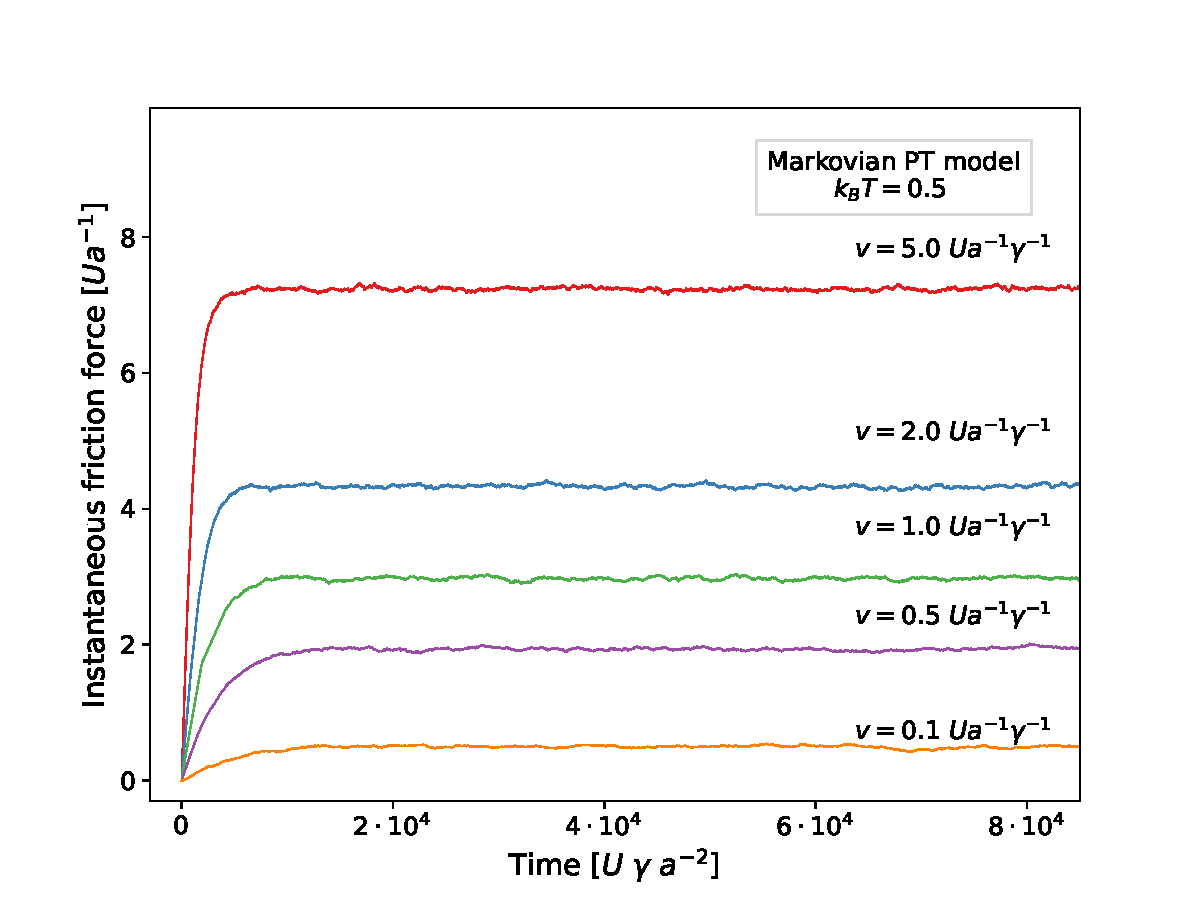
\includegraphics[width=\textwidth]{alteV_kb0_forzaplot.pdf}
    \caption{Instantaneous friction force for a few driving velocities $v$ in the standard Markovian PT model.}
    \label{fig:friction_kb0_high_velocities}
\end{figure}
In the Prandtl-Tomlinson model, the friction force can be evaluated from the elastic force associated with the elongation of the spring coupling the slider to the colloidal particle. This elastic force is described by the equation
\begin{equation}
    F_k(v,t) = K\Delta x = K (x_\text{slider} - x) = K(vt -  x)\; .
\end{equation}
Here the slider position $x_\text{slider}$ is simply given by the product of its constant velocity and time.

Figure \ref{fig:friction_kb0_high_velocities} compares the time dependence of the instantaneous friction forces in the standard Prantl-Tomlinson model, using $K=0.001\;Ua^{-2}$, amplitude $2U$ and lattice spacing $a$, for a few values of velocity, from $v=0.1\hspace{0.1cm}U\gamma^{-1} a^{-1}$ to $v=5\hspace{0.1cm}U\gamma^{-1} a^{-1}$. 
\begin{figure}[ht!]
    \centering
    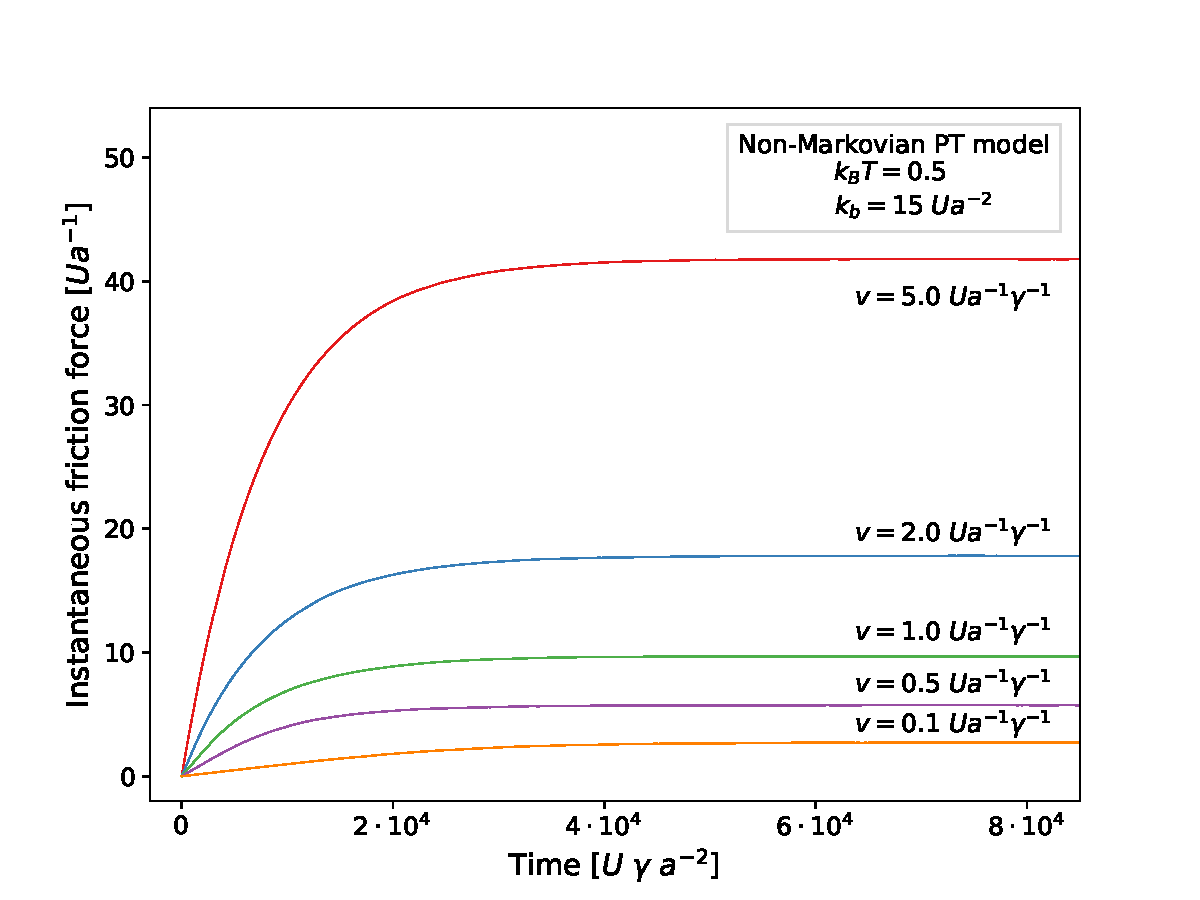
\includegraphics[width=\textwidth]{alteV_kb15_forzaplot.pdf}
    \caption{Instantaneous friction force for a few driving velocities $v$ in the non-Markovian PT model with $k_b=15\; Ua^{-2}$.}
    \label{fig:friction_kb15_high_velocities}
\end{figure}

Similarly, Figure \ref{fig:friction_kb15_high_velocities} compares the friction forces in the non-Markovian PT model as a function of time for the same driving velocities, and for $k_b=15\hspace{0.1cm}Ua^{-2}$.
In both these two figures, it is evident that initially the particle lags many length units behind the tracer.

This initial transient needs to be omitted in the evaluation of the time-averaged friction: we compute the average force starting after the end of the transient, when the force stabilizes. As recalled above, in this regime, for the standard overdamped PT model, the dependence of the friction force on velocity is linear, as verified in Figure \ref{fig:high_velo_friction}. The non-Markovian PT model too exhibits a linear dependence on velocity, but with a much larger slope,the result of the coupling with an environment characterized by a higher dissipation coefficient $\gamma_b$ compared to that of the particle $\gamma$.
\begin{figure}
    \centering
    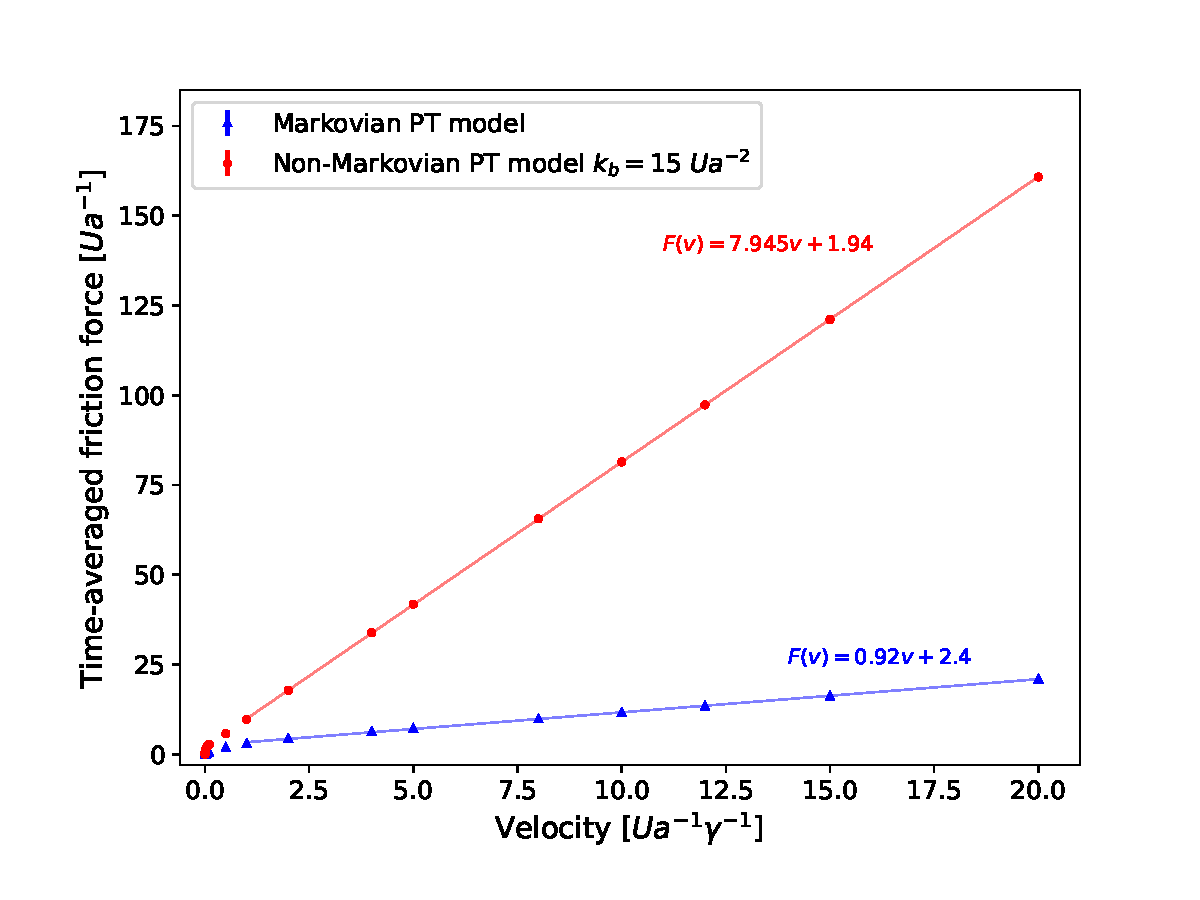
\includegraphics[width=\textwidth]{tot_lineare.pdf}
    \caption{Time-averaged friction force velocity-dependence. Dot-dashed line: the $T=0$ static friction.}
    \label{fig:high_velo_friction}
\end{figure} 
We fit the friction data for $v \geq \hspace{0.1cm}Ua^{-1}\gamma^{-1}$  with this linear expression
\begin{equation}
    F(v)=F_0 + \gamma^{*} v \, ,
    \label{eq:lin_fit}
\end{equation}
and report the resulting best-fit coefficients in Table \ref{tab:valori_gammaeff}.
\begin{table}
\centering 
\begin{tabular}{ccc}
    \toprule
    $k_b$ [$U a ^{-2}$] & Slope $\gamma^{*}$  [$\gamma$]& Intercept  $F_0$ [$U a ^{-1}$]\\
    \midrule 
    $0$ & $0.92 \pm 0.02$ & $2.4 \pm 0.1$\\
    $15$ & $7.945 \pm 0.003$ & $1.94 \pm 0.01 $\\
    \bottomrule
\end{tabular}
\caption{Best-fit coefficients for the linear velocity-dependence of friction force at high velocity, according to Eq.\;\eqref{eq:lin_fit}.}
\label{tab:valori_gammaeff}
\end{table}
\\
Notice that the value of $\gamma^*$ in the standard Prandtl-Tomlinson model is slightly lower than the thermostat parameter $\gamma$. This is the result of thermal fluctuations that help the particle to escape the potential wells, with the result that friction is smaller than one expects for the $T=0$ PT model. On the other hand, the non-Markovian PT model, shows an effective damping coefficient $\gamma^* \lesssim \gamma + \gamma_b$, thus slightly lower than the sum of the friction coefficients of the colloidal particle and of the viscoelastic bath particle.
\begin{figure}
    \centering
    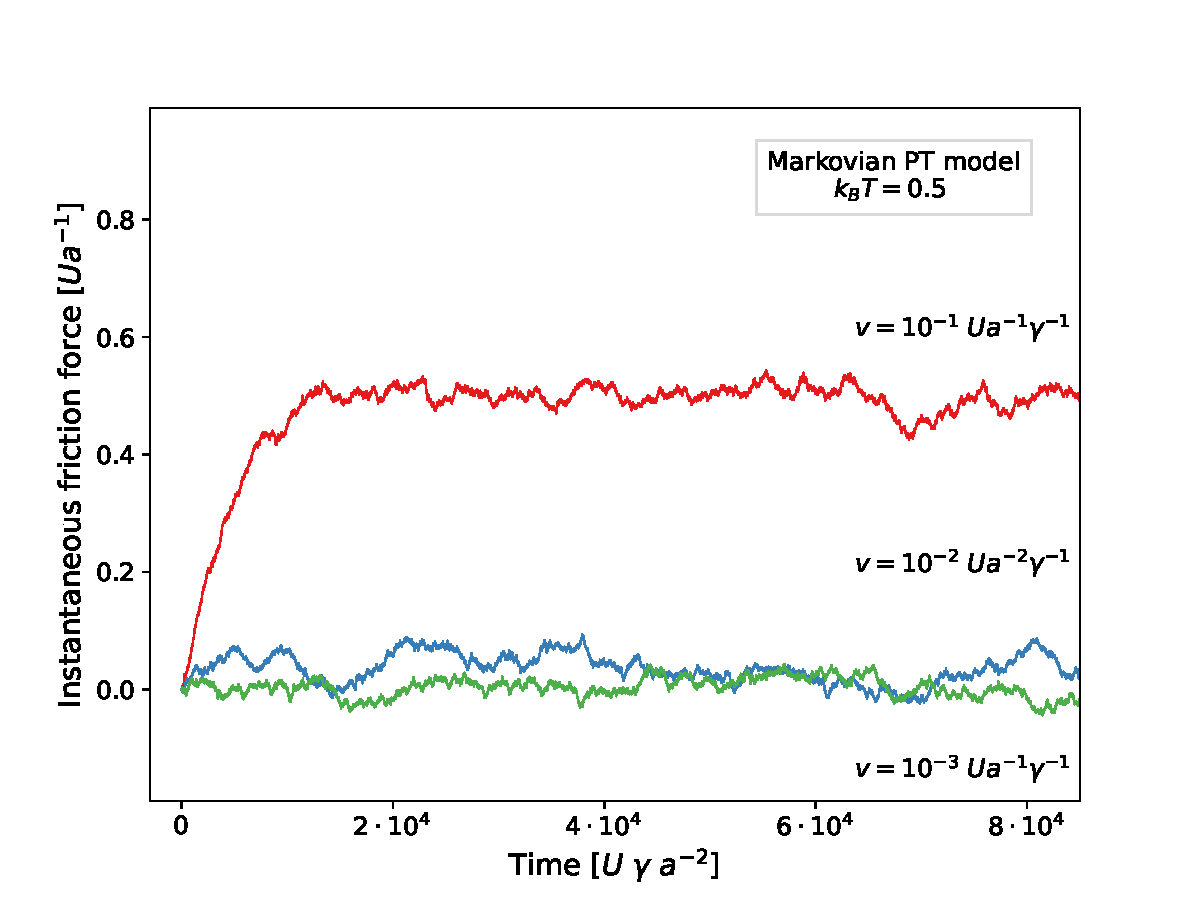
\includegraphics[width=\textwidth]{basseV_kb0_forzaplot.pdf}
    \caption{Friction force as a function of time in the Markovian PT model, in the low-velocity regime }
    \label{fig:basseV_kb0_friction}
\end{figure}
Regarding the velocity-dependence of the friction force in the more interesting low velocity regime, we conduct only a preliminary study is conducted due to subtle difficulties associated to numerical data analysis. Specifically at very low velocity, under $10^{-3}\hspace{0.1cm}U\gamma^{-1} a^{-1}$, the effects of stochastic thermal forces cause the particle to jump from one minimum to another, with the dragging-forward dynamics remaining a minor, perturbative effect. Figure \ref{fig:basseV_kb0_friction} illustrates how already at $v \simeq 10^{-2}\hspace{0.1cm}U\gamma^{-1} a^{-1}$ or $10^{-3}\hspace{0.1cm}U\gamma^{-1} a^{-1}$, the friction force fluctuates widely: these fluctuations are comparable in size to the average friction force itself, or even larger. As a result, extracting a significant friction force from the time average rapidly becomes a formidable task, that would require extremely long simulations to average out the thermal noise.

For $v<0.01\; U\gamma^{-1}a^{-1}$ outlined above where diffusion dominates over driving, we choose to perform a time averaging without omitting any transient, which is not well-defined, and to carry it out over the entire simulation time, which we extend from a minimum $10^6 \hspace{0.1cm}t_0$ up to $2 \cdot 10^7 \hspace{0.1cm}t_0$, depending on the slider velocity. This choice is made for the standard Prandtl-Tomlinson situation, which can be seen in Figure \ref{fig:basseV_kb0_friction}.
\begin{figure}
    \centering
    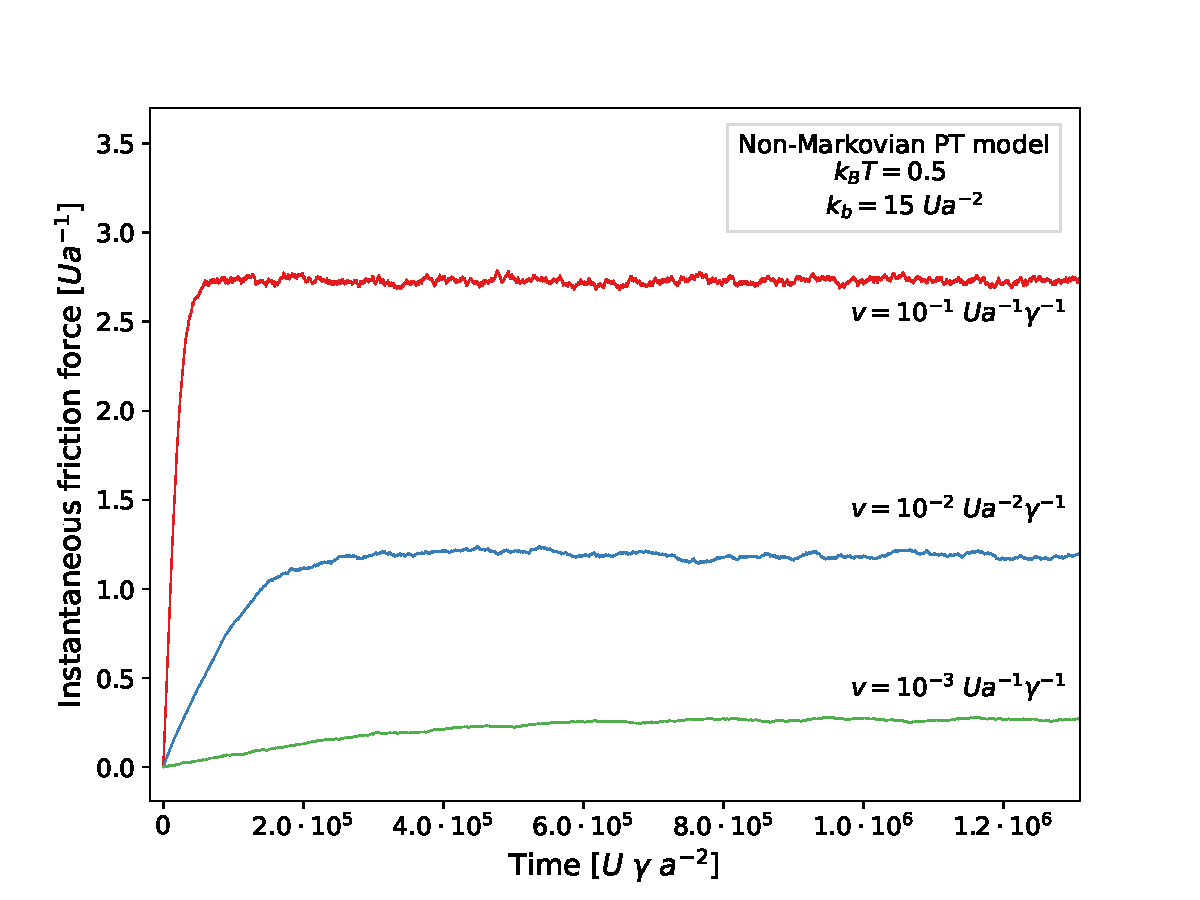
\includegraphics[width=\textwidth]{basseV_kb15_forzaplot.pdf}
    \caption{Friction force as a function of time in the non-Markovian PT model, in low velocity regime.}
    \label{fig:basseV_kb15_friction}
\end{figure}
\\
In the scenario of non-Markovian Prandtl-Tomlinson, Fig. \ref{fig:basseV_kb15_friction}, due to the coupling with a more strongly damped environment, the friction force is more stable over time. This leads to a more reliable and computationally simpler determination of its value even in the low-velocity regime. This figure allows us to appropriately select the transient part to be excluded from the temporal averaging of the friction forces. It is observed that this quantity increases significantly as the velocity decreases, reaching $10^6\hspace{0.1cm}  t_0$ for $v=10^{-3} \hspace{0.1cm} Ua^{-1}\gamma^{-1}$.

Figure \ref{fig:totale_logartimX} compares the velocity dependence of the time-averaged friction force for both the Markovian and non-Markovian PT models as a function of the driving velocity in $\log{(v)}$ scale, across a broad velocity range. This figure also includes the value of the static friction force $F_\text{static}$ calculated in Section \ref{ourmodel}.
\begin{figure}
    \centering
    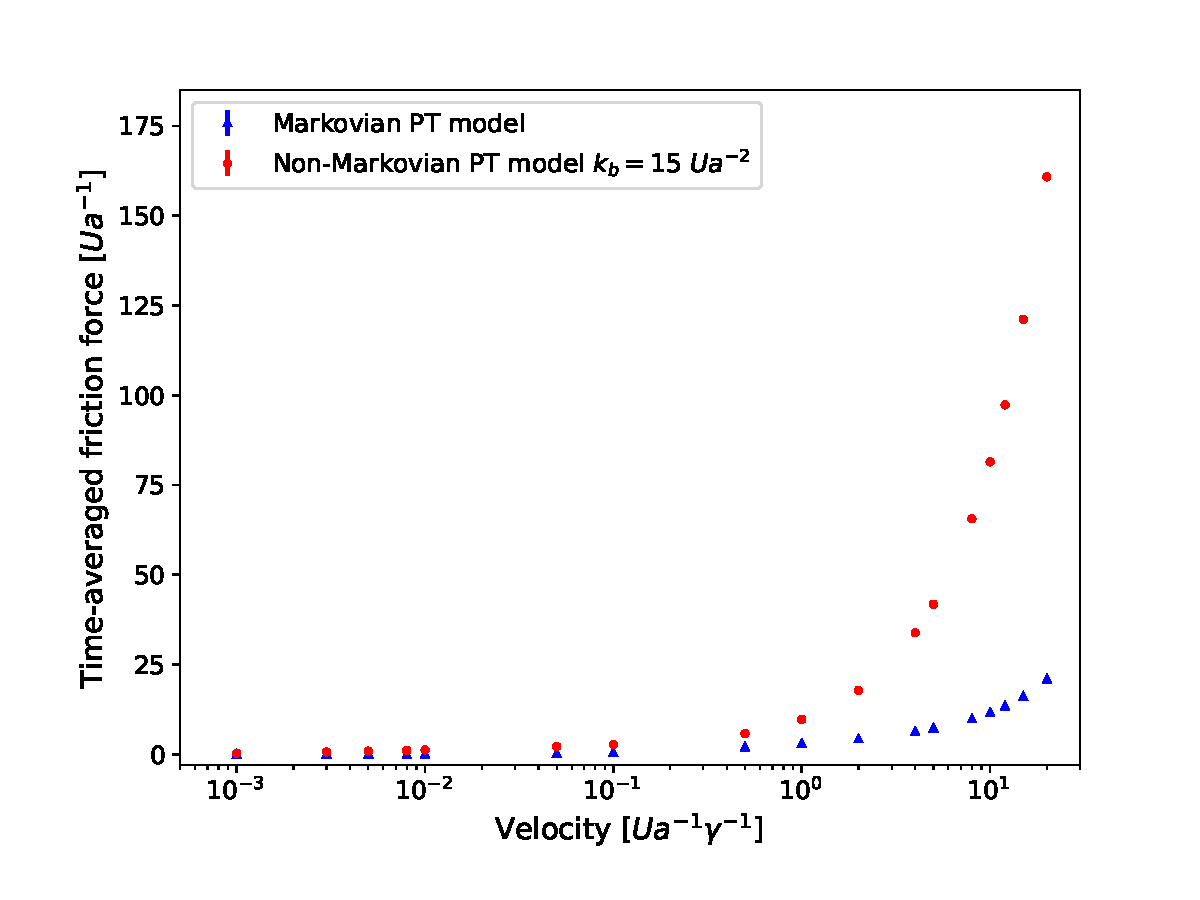
\includegraphics[width=\textwidth]{tot_logaritmica.pdf}
    \caption{Same as Fig.~\ref{fig:high_velo_friction}, but with velocity in logarithmic scale.}
    \label{fig:totale_logartimX}
\end{figure} We observe that in the low-velocity regime, the time-averaged friction force deviates from the linear variation appropriate for large velocity, but exhibits a much slower variation. For the standard PT over a limited range, the expected velocity-dependence is verified (Fig. \ref{fig:low_velocities}) with a curve fit in the following form  
\begin{equation}
    F(v) = f - a \log{\left(\dfrac{b}{v}\right)}^\frac{2}{3}\; ,
\end{equation}
Table \ref{tab:param_lowvel} reports the best-fit parameters.
\begin{table}
\centering
\begin{tabular}{ccc}
    \toprule
    \multicolumn{3}{c}{Fit parameters} \\
    \midrule
   $f$ [$Ua^{-2}$] &  $a$ [$Ua^{-2}$] & $b$ [$Ua^{-1}\gamma^{-1}$] \\
    \midrule 
    $0.03 \pm 0.02$ & $0.05\pm 0.03$ & $0.010 \pm 0.001$ \\
    \bottomrule
\end{tabular}
\caption{Best-fit coefficients for the velocity-dependence of friction force in low-velocity regime.}
\label{tab:param_lowvel}
\end{table}
For the non-Markovian PT model Figure \ref{fig:low_velocities} indicates that it may be necessary to repeat the calculations for smaller velocity $v$ to verify the low-speed behavior of the model.
\begin{figure}
    \centering
    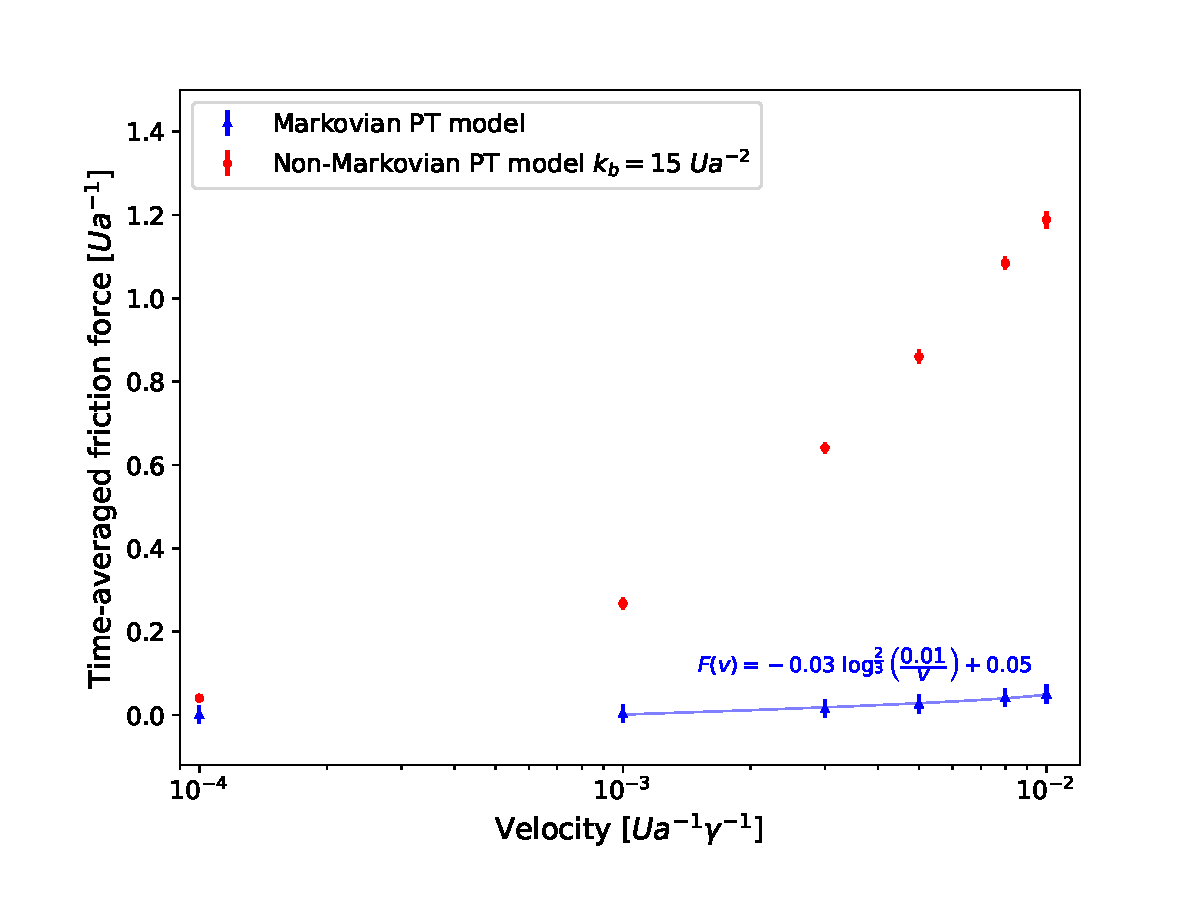
\includegraphics[width=\textwidth]{lowvelocities.pdf}
    \caption{Same as Fig.~\ref{fig:totale_logartimX}, detail of the low-velocity range.}
    \label{fig:low_velocities}
\end{figure}

\newpage
\chapter{Conclusions and Outlook}
In this thesis we investigate the overdamped dynamics of a colloidal particle in a viscoelastic bath, namely an environment characterized by memory
effects. From our simple implementation to include a non-Markovian environment in the Prandtl-Tomlinson model, some results and considerations for future developments have emerged, which we summarize here. 

We found that the effect of the viscoelastic bath is an increase of the potential barrier experienced by the particle compared to the standard Brownian case.
This increase of the effective barriers affects the waiting-time distributions. This effect is clearly visible at the level of the distribution resulting from standard Brownian diffusion and non-Markovian Brownian diffusion. In the standard PT model the waiting-time distribution follows an exponential decay. Instead, in the non-Markovian case, we observe a sum of two exponentials, with two radically different characteristic times. At short times, the distribution exhibited a very rapid decay reflecting the fast barrier crossing events caused by the coupling with the viscoelastic bath. In the longer timescale, the distribution shows that the particle can remain in a potential well for many time units before a barrier crossing event occurrs. Our study reveals how a stronger coupling of the particle with the viscoelastic bath leads to an increase in the characteristic time on the long timescale, whereas on the short timescale, the characteristic time is reduced due to the larger restoring force exerted by the bath particle. Furthermore, we observe that the characteristic long timescale decreases with increasing temperature. 

The waiting-time distributions for the standard Prandtl-Tomlinson model and for its non-Markovian extension at finite driving velocity are also quite instructive. Specifically a non-monotonic distribution, with a peak forming around the typical time spent in a potential minimum, determined by the ratio $a/v$ (the washboard frequency) between the distance of two consecutive minima and the dragging velocity.

The main nontrivial features brought to the waiting-time distribution by the non-Markovian model are: (i) the survival of a short-time fast exponential decay related to the fast back-and-forth events promoted by the viscoelastic nature of the thermostat; (ii) a far slower exponential decay of long residence times compared to the regular memory-free model. A separation between the forward (rightward) and backward (leftward) jump events also shows a quite distinct features brought by the memory thermostat.

Finally, we carried out a preliminary investigation of the velocity dependence of the time-averaged friction force in both the standard PT model and its non-Markovian extension. We covered in some detail the trivial high-velocity regime, where both exhibit a linear trend, albeit with a different slope, associated to the extra viscosity brought in by the fake particle modeling viscoelastic effects. We also carried out a preliminary analysis of the low-velocity regime, which proves to be more computationally challenging.

This thesis provides a few important, but preliminary milestones to the investigation of memory effects in the PT model.

We have shown that the simple addition of the viscoelastic bath increases both the effective corrugation, relevant at low velocity, but also the high-velocity viscous friction. For a fair comparison with regular memory-free model an important step will require determining a recipe for the model parameters that would allow a fair comparison of the two thermostats. 

Once this task is achieved, several extension of the present investigation are envisageable. In particular it will be interesting to verify if in the small-velocity regime the regular logarithmic dependence of friction on velocity is retained or modified. However for this task very long simulations will be necessary.

\printbibliography

\chapter*{Ringraziamenti}

\textit{Un accorato ringraziamento è rivolto al prof.\,Manini, la cui disponibilità e professionalità hanno reso staordinaria la fine di questo percorso accademico.}
\\
    \textit{Ringrazio i miei amati nonni e la mia famiglia tutta; il vostro sostegno e amore sono e saranno sempre impareggiabili.}
    \\
    \textit{Grazie a tutti i ragazzi di Fisica, una seconda famiglia.}
    \\
    \textit{Un accorato ringraziamento è rivolto al prof.\,Manini, la cui disponibilità e professionalità hanno reso staordinaria la fine di questo percorso accademico.}
    \vspace{1cm}
    \\
    \textit{Grazie a via Celoria 16, 
    \\
    mia seconda casa, 
    \\
    sempre.}
    \vspace{0.5cm}
    \\
    \begin{flushright}
        \textit{Stefano}
    \end{flushright}
\end{document}